\section{Experimental Analysis}\label{s:exp}

We now evaluate our \esp{} methods on representative real-world datasets of
varying density and label regularity.
After presenting the data and our evaluation criterion, we proceed in two steps. First, we simulate
our generative model on real networks to give them signs, then we study to which extent we can recover
the parameters $p$ and $q$ of each node, and how predictions based on these estimation compare with
the Bayes optimal. Second, we select random training sets from the actual signs.
This shows that our methods compete well against
existing approaches in terms of both predictive and computational performance. We are especially
interested in small training set regimes, and have restricted our comparison to the batch learning
scenario since all competing methods we are aware of have been developed in that setting only.

\subsection{Datasets}

We consider six real-world classification datasets. The first four are \dssn{} widely
used as benchmarks for this
task~(\eg{}\autocites{Leskovec2010}{shahriari2014ranking}{wu2016troll}{OnlineCompletion17}):
In \adv{}, a trust-based social network for open source developers, a user $u$ can certify another
user $v$ with different degrees of trust: \enquote{Observer}, \enquote{Apprentice} (both of which we
consider negative), \enquote{Journeyer} and \enquote{Master} (both of which we consider
positive).\footnote{We download the 7\thup{} of July, 2014 version from
\url{http://www.trustlet.org/datasets/advogato/}.} A full description of this trust metric, and its
resistance to attacks, is available in the PhD thesis of the website's creator~\autocite[Section
4]{AdvogatoTrustThesis02}).
In \wik{}, there is an edge from user $u$ to user $v$ if $v$ applies for an admin position and $u$
votes for or against that promotion. In \sla{}, a news sharing and commenting website, member $u$
can tag other members $v$ as friends or foes. Finally, in \epi{}, an online shopping website, user
$v$ reviews products and, based on these reviews, another user $u$ can display whether he considers
$v$ to be reliable or not. In addition to these four datasets, we considered two other \ssn{} where
the signs are inferred automatically, rather than given explicitly by the users.  In
\kiw{}~\cite{wikiedits11}, an edge from Wikipedia user $u$ to user $v$ indicates whether they edited
the same article in a constructive manner or not.\footnote{This is the
\href{http://konect.uni-koblenz.de/networks/wikisigned-k2}{KONECT version of the
\enquote{Wikisigned} dataset}, from which we removed self-loops.} Finally, in the
\aut{}~\cite{kumar2016structure} network, an author $u$ cites another author $v$ by either endorsing
or criticizing $v$'s work. The edge sign is derived by classifying the citation sentiment with a
technique using a list of positive and negative words; see
\cite{kumar2016structure} for more details.\footnote{We again removed self-loops and merged
multi-edges which are all of the same sign.}

\begin{table}[bt]
  \centering
  \small
  \caption{Dataset properties. The 5\thup{} column gives the fraction of positive labels. The next two
  columns provide two different measures of label regularity, while the last two columns give the
  proportion of reciprocal edges, and among them the fraction with different signs.\label{tab:dataset}}
  \begin{tabular}{lrrrrrrrr}
    \toprule
    Dataset & \thead{$|V|$}       & \thead{$|E|$}       & \thead{$\frac{|E|}{|V|}$} &
    \thead{$\frac{|E^+|}{|E|}$} & \thead{$\frac{\Psi^2_{G''}(Y)}{|E|}$} &
    \thead{$\frac{\Psi_G(Y)}{|E|}$} & \thead{reciprocal\\ edges} &
    \thead{reciprocal\\ disagreement} \\
    \midrule                                                                                                   
    \aut{}  & \np{4831}   & \np{39452}  & 8.2               & 72.3\%              & .076                          & .191                    & 5.1\%      & 27.1\%            \\
    \adv{}  & \np{5417}   & \np{51312}  & 9.5               & 75.1\%              & .061                          & .132                    & 33.6\%     & 28.6\%            \\
    \wik{}  & \np{7114}   & \np{103108} & 14.5              & 78.8\%              & .063                          & .142                    & 5.6\%      & 10.0\%            \\
    \sla{}  & \np{82140}  & \np{549202} & 6.7               & 77.4\%              & .059                          & .143                    & 17.7\%     & 4.0\%             \\
    \epi{}  & \np{131580} & \np{840799} & 6.4               & 85.3\%              & .031                          & .074                    & 30.8\%     & 2.1\%             \\
    \kiw{}  & \np{138587} & \np{740106} & 5.3               & 87.9\%              & .034                          & .086                    & 6.5\%      & 14.6\%            \\
    \bottomrule
  \end{tabular}
\end{table}

\autoref{tab:dataset} summarizes statistics for these datasets. We note that most edge labels are
positive. Hence, test set accuracy is not an appropriate measure of prediction performance. We
instead evaluated our performance using the so-called Matthews Correlation Coefficient
(MCC)~\autocite{MCC00}, defined as
\begin{equation}
  \label{eq:troll_mcc}
	\mathrm{MCC} = \frac{tp\times tn-fp\times fn}%
        {\sqrt{ (tp + fp) ( tp + fn ) ( tn + fp ) ( tn + fn ) } }% = \pm \sqrt{\frac{\chi^2}{n}}
\end{equation}
MCC combines all the four quantities found in a binary confusion matrix ($t$rue $p$ositive, $t$rue
$n$egative, $f$alse $p$ositive and $f$alse $n$egative) into a single metric which ranges from $-1$
(when all predictions are incorrect) to $+1$ (when all predictions are correct) through $0$ (when
predictions are made uniformly at random).

Although the semantics of the edge signs is not the same across these networks, we can see from
\autoref{tab:dataset} that our generative model essentially fits all of them. Specifically,
two columns of the table report the rate of label (ir)regularity, as measured by
$\Psi^2_{G''}(Y)/|E|$ (6\thup{} column) and $\Psi_{G}(Y)/|E|$ (7\thup{} column), where 
\[
  \Psi^2_{G''}(Y) = \min_{(\bp,\bq)} \sum_{(u,v) \in E}
  \left(\frac{1+\yuv}{2} - \frac{p_u+q_v}{2} \right)^2
\]
as first described in \autoref{ss:passive}
and $\Psi_{G}(Y)$ is the
label regularity measure adopted in the online setting, as defined in \autoref{s:prel}. It is
reasonable to expect that higher label irregularity corresponds to lower prediction performance.
This trend is in fact confirmed by our experimental findings: whereas \epi{} tends to be easy,
\aut{} tends to be hard, and this holds for all algorithms we tested, even if they do not explicitly
comply with our inductive bias principles. Moreover, $\Psi^2_{G''}(Y)/|E|$ tends to be proportional
to $\Psi_{G}(Y)/|E|$ across datasets, hence confirming the anticipated connection between the two
regularity measures.

Finally, there is a low fraction of reciprocal edges (\ie{} both $\euv \in E$ and $\evu
\in E$), which is a common mechanism of link formation in directed
networks~\autocites{DirectedReciprocity04}{Reciprocity13}). Moreover, in most cases, such reciprocal edges do not disagree,
\ie{} they have the same sign. In practice, we can use this fact to improve our accuracy at no
additional computational cost: when predicting $\euv \in E_{\mathrm{test}}$, if the reciprocal edge
\evu{} is part of the training set, we set $\yhat_{u,v} = y_{v,u}$. For clarity, when comparing
our methods with existing approaches, we not use that trick. But afterwards, we show in
\autoref{tab:twin} when it can be beneficial.
% more references in  http://www.nature.com/articles/srep02729

\subsection{Synthetic signs}

Recall that according to our generative model of \autoref{s:gen}, each node $u$ has a parameter $p_u$
governing its sending behavior and each node $v$ has a parameter $q_v$ governing its receiving
behavior, such that the sign of the edge \euv{} is positive with probability $\frac{p_u+q_v}{2} =
\etauv$. Given a topology $G=(V,E)$, we start by assigning a $p$ and $q$ values to each node. If we
want \etauv{} to be uniform over $E$, we have to take into account the out-degree of nodes with at
least one outgoing edge, and likewise the in-degree of nodes with at least one incoming edge. For
that, in the case of $p$, we partition the interval $[0,1]$ into $|V|$ segments of size proportional
to $\dout(u_1),
\dout(u_2), \ldots, \dout(u_{|V|})$. We shuffle these segments and draw a number \uar{} from each of
them, which we set as the initial $p'$ value of the corresponding node. Then, because we want to model real
sign distribution and have more
positive than negative edges, we apply an exponential transformation \[ p = \frac{1}{1-e^{-\lambda}}
\left( 1-e^{-\lambda p'} \right) \,,\] where we choose $\lambda=3$. We do the same for $q$, then for
every edge \euv{}, we set it positive with probability \etauv{}. An example of the distributions we
obtain for the \wik{} graph is showed on \autoref{fig:troll_synth_distrib}\footnote{More precisely,
these figures are normalized histogram, meaning the counts are scale down so that the bars total
area sums up to one.}, giving $71.9\%$ of positive edges.

% TODO: do a proper subfigure instead of minipage?
\vspace{\baselineskip}
\noindent\begin{minipage}{187mm} 
  \begin{minipage}{46mm}
    \centering
    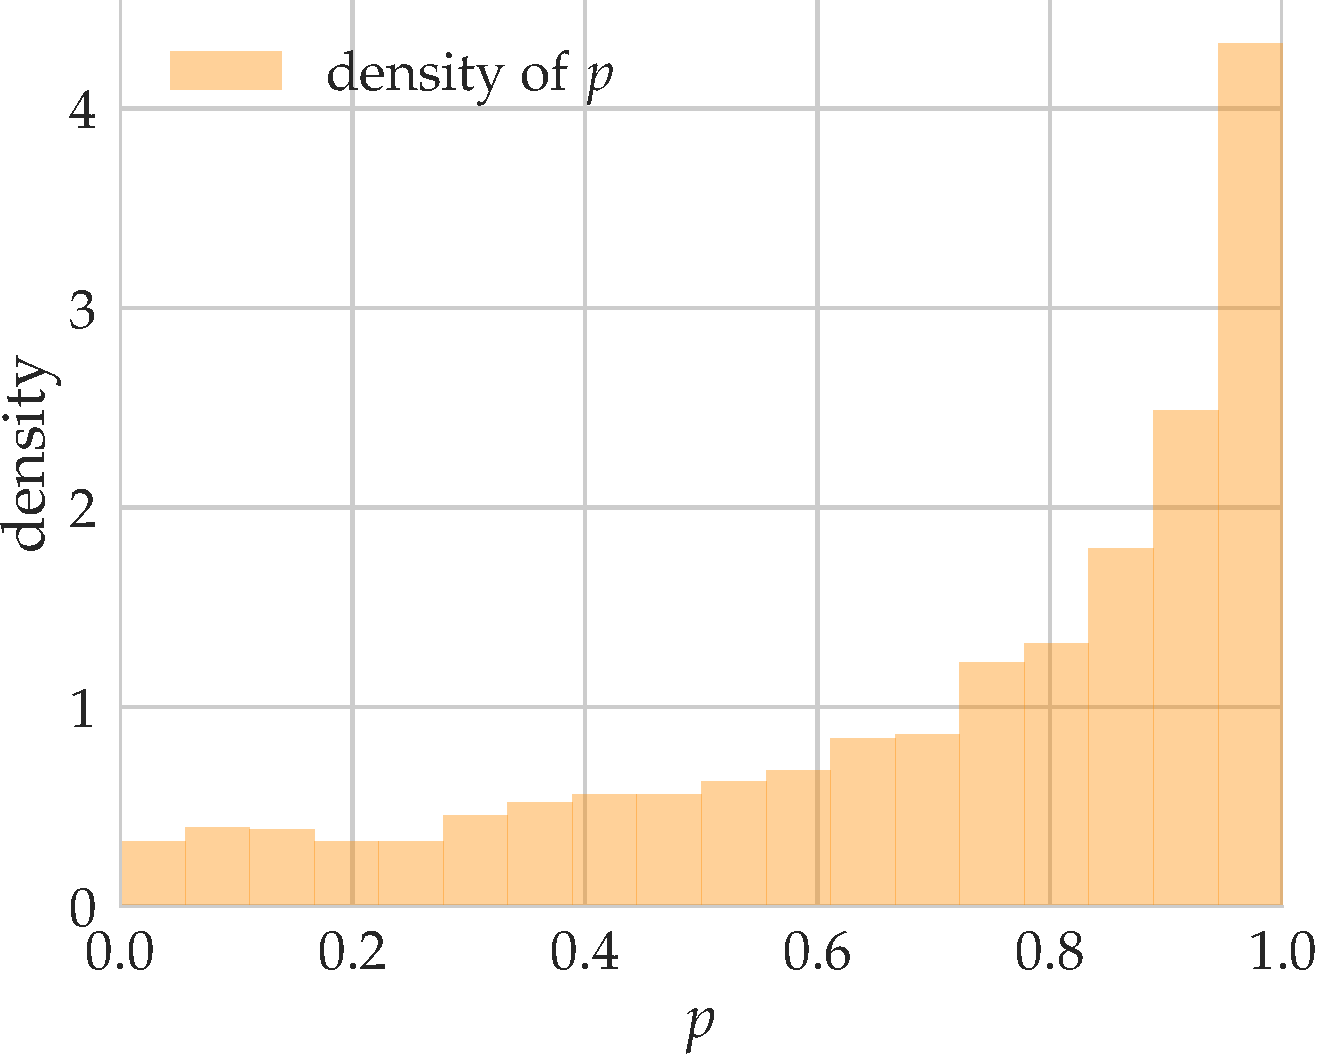
\includegraphics[width=.95\linewidth]{raw/synth_wik_pdense.pdf}
    \captionof{subfigure}{Density of $p$.}
    % \label{fig:figure1}
  \end{minipage}%
  \begin{minipage}{46mm}
    \centering 
    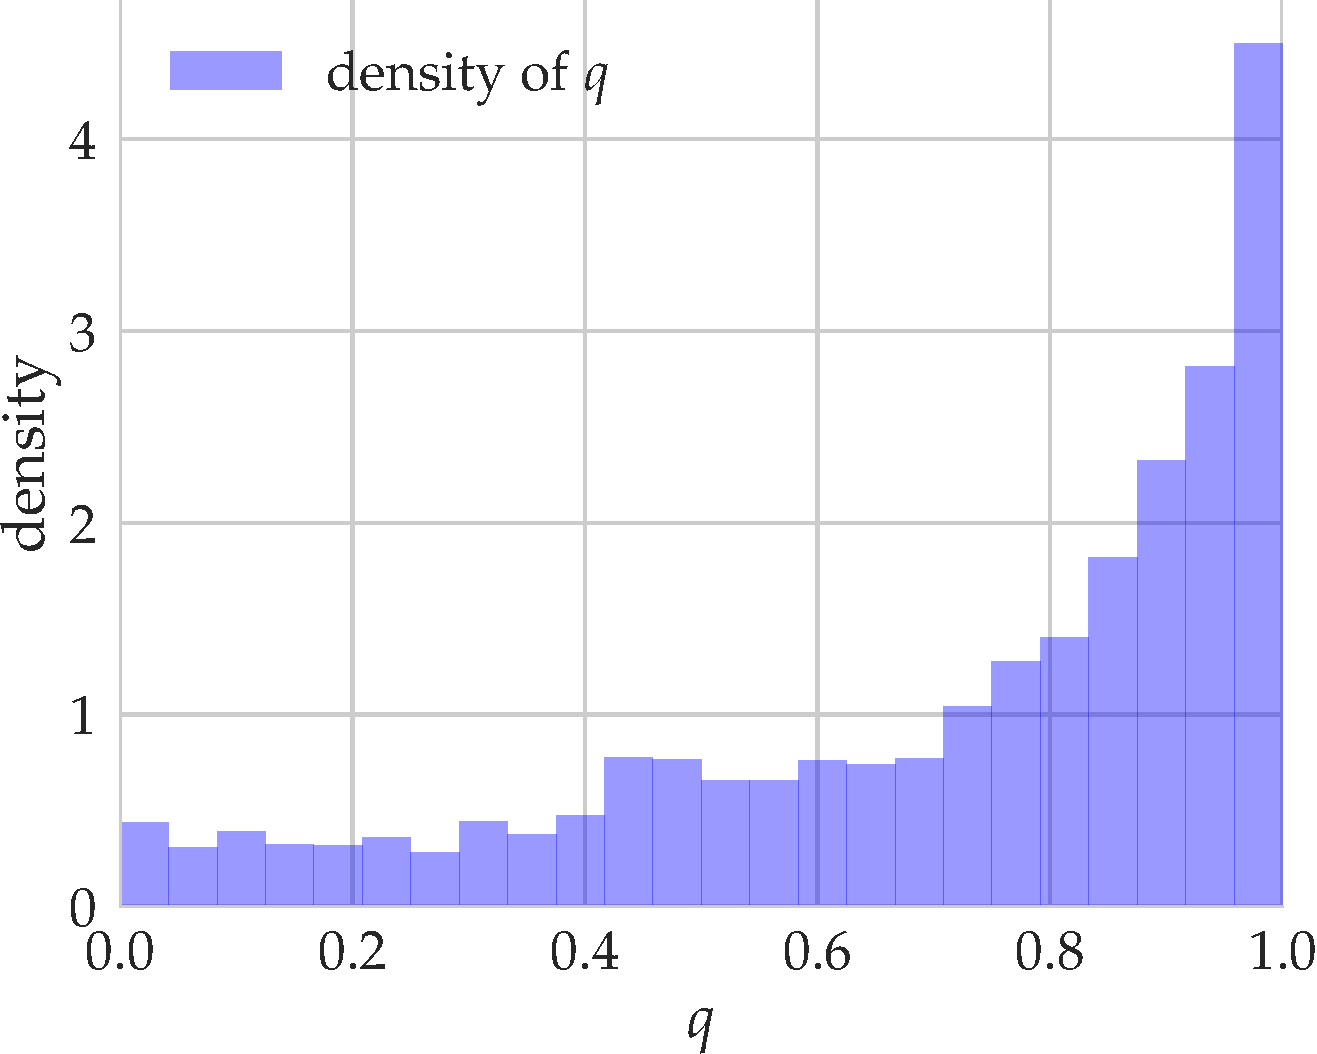
\includegraphics[width=.95\linewidth]{raw/synth_wik_qdense.pdf} 
    \captionof{subfigure}{Density of $q$.} 
    % \label{fig:figure2} 
  \end{minipage} 
  \begin{minipage}{46mm}
    \centering 
    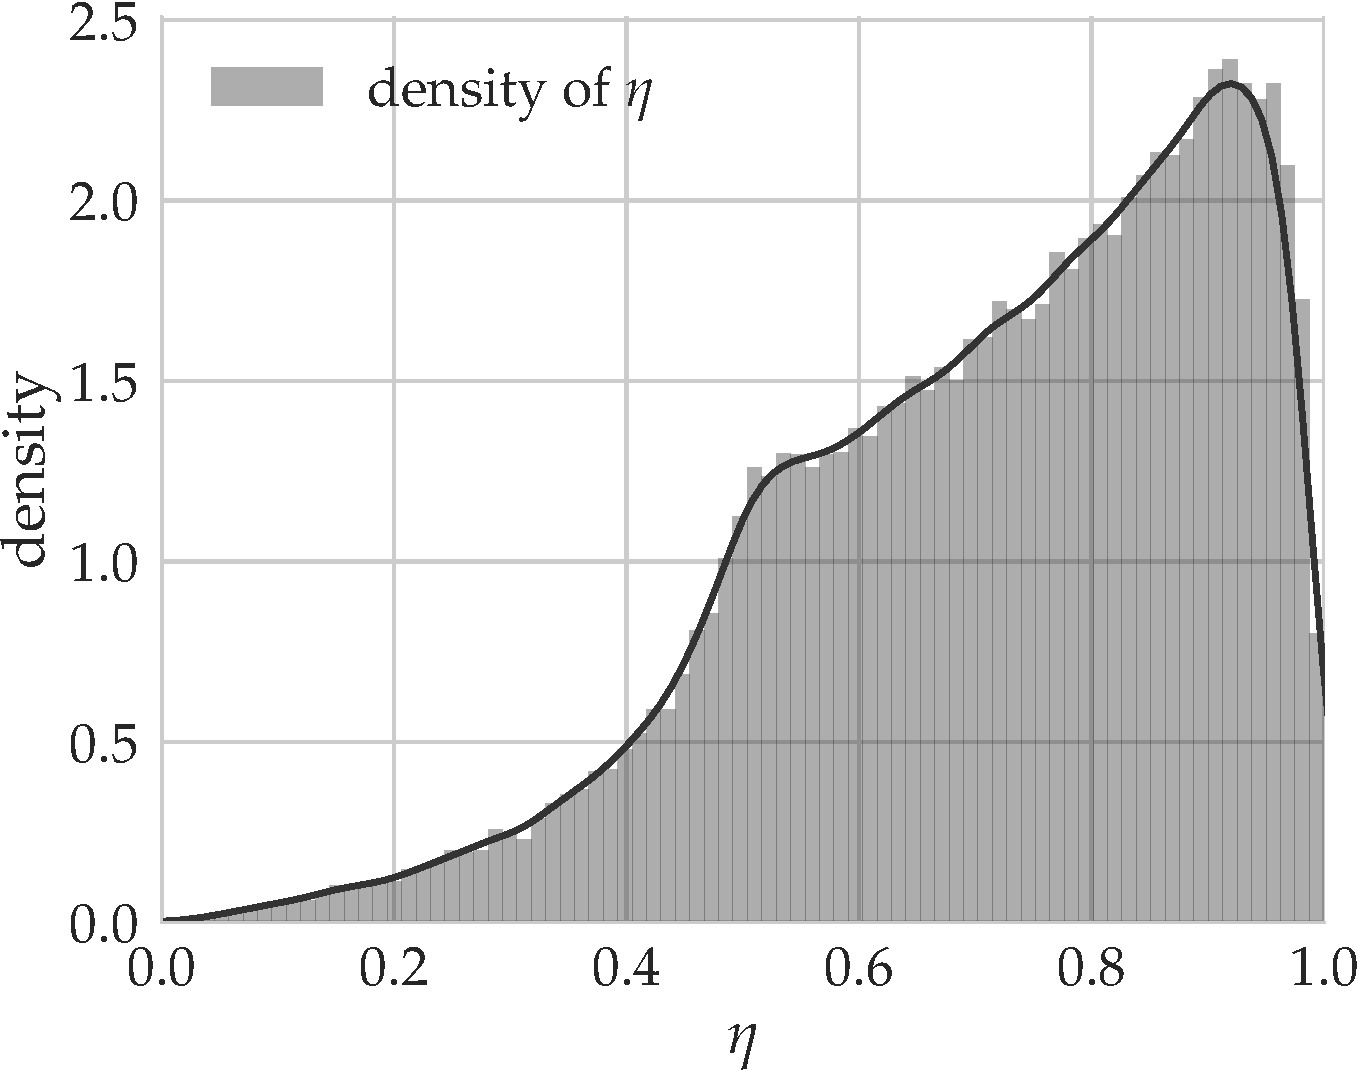
\includegraphics[width=.95\linewidth]{raw/synth_wik_etadense.pdf} 
    \captionof{subfigure}{Density of $\eta$.} 
    % \label{fig:figure2} 
  \end{minipage} 
  \begin{minipage}{46mm}
    \centering 
    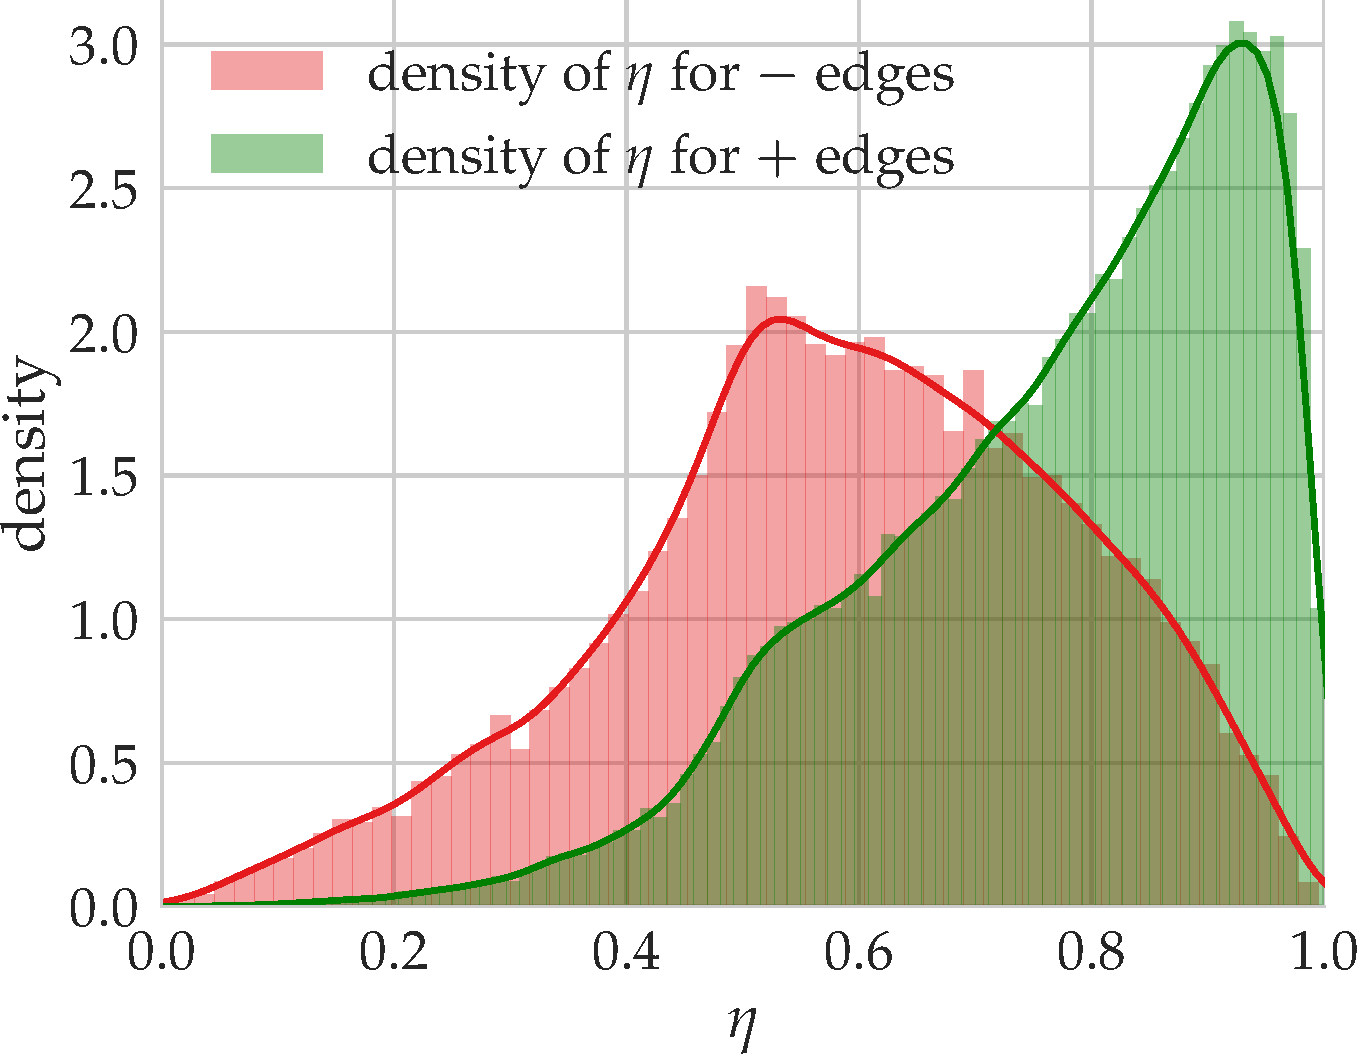
\includegraphics[width=.95\linewidth]{raw/synth_wik_signdense.pdf}
    \captionof{subfigure}{Density of $\eta$ for both signs.} 
    % \label{fig:figure2} 
  \end{minipage} 
  \captionof{figure}{Synthetic distributions on \wik{}.} 
  \label{fig:troll_synth_distrib} 
\end{minipage}
\vspace{\baselineskip}

Once the signs are generated, we select a training set \trainset{} \uar{}, and predict
the signs of the remaining edges in the testing set $E\setminus \trainset{}$. The Bayes optimal
predictor classifies an edge \euv{} as positive if $\etauv \geq \shalf$ and negative otherwise. 
We compare it with the \usrule{} algorithm analyzed in \autoref{ss:bayes_approx}. Recall that
\usrule{} proceeds as follow: after computing $\htr(u)$ and $\hun(u)$ on training set $E_0$ for all
$u \in V$ (or setting those values to \shalf{} in case there is no outgoing or incoming edges for
some node), we use the equation \eqref{eq:predictor}\footnote{We reproduce this equation here for
convenience: $\sgn\Big(\big(1-\htr(u)\big) + \big(1-\hun(v)\big) -\tau - \tfrac{1}{2}\Big)$.},
having estimated $\tau$ on $E_0$.

The result of this comparison on the six datasets is showed in \autoref{tab:troll_synth_global}.
For each network, we generated the signs once. Then, for different training size (20\%, 40\% or 80\%
of $E$), we sampled a training set and predict using the knowledge of the true $\eta$ (Bayes
predictor) or its estimated value (\usrule{}).
The MCC of the Bayes predictor is the same on all datasets (around $30$\footnote{Here and in the
following, we multiply all MCC value by 100 to improve readability.}), and so is its accuracy
(around $75\%$). The corresponding values for \usrule{} are close on all datasets (although some are
easier) and the gap naturally decreases as the training size increases. Another interesting
quantity is how close can \usrule{} estimates $\eta$ using $\wh{\eta} = \left(1-\htr(u)\right) +
\left(1-\hun(v)\right) -\tauhat$ as defined in \autoref{ss:bayes_approx}. We compute the mean
absolute error (MAE) between $\eta$ and $\wh{\eta}$ for all testing edges, and then specifically for
the testing edges whose both endpoints have been sampled above a certain threshold in the training
set. As expected, the estimation is more accurate with increasing training set size, and with
increasing number of samples for a given edge.

\begin{center}
  \small
  \captionsetup{font=small}
  \captionof{table}{%
    The results are averaged over 25 random sampling of \trainset{}.
    \label{tab:troll_synth_global}
  }
  \begin{longtable}{llrrrrrr}
    \toprule
    \thead{Dataset} & \thead{$\frac{|\trainset{}|}{|E|}$}
                    & \thead{\usrule{}\\ Accuracy}   & \thead{Bayes\\ Accuracy}
                    & \thead{\usrule{}\\ MCC}        & \thead{Bayes\\ MCC}
                    & \thead{MAE$(\eta, \wh{\eta})$\\ testing set} & \thead{MAE$(\eta, \wh{\eta})$\\ many samples} \\
\midrule
\multirow{3}{*}{\aut{}} & 20\% & $66.1\pm0.6$ & $75.1\pm0.1$ & $16.2\pm0.5$ & $29.7\pm0.2$ & $.256\pm.00$ & $.119\pm.01$ \\
                        & 40\% & $68.2\pm0.4$ & $74.7\pm0.2$ & $19.1\pm0.6$ & $29.6\pm0.4$ & $.205\pm.00$ & $.085\pm.00$ \\
                        & 80\% & $71.4\pm0.4$ & $75.1\pm0.5$ & $23.4\pm0.9$ & $29.7\pm1.1$ & $.152\pm.00$ & $.059\pm.00$ \\
\midrule
\multirow{3}{*}{\adv{}} & 20\% & $66.5\pm0.6$ & $75.1\pm0.1$ & $17.1\pm0.6$ & $30.3\pm0.2$ & $.242\pm.00$ & $.116\pm.00$ \\
                        & 40\% & $69.6\pm0.4$ & $75.4\pm0.1$ & $21.0\pm0.5$ & $30.8\pm0.3$ & $.192\pm.00$ & $.083\pm.00$ \\
                        & 80\% & $71.6\pm0.5$ & $75.4\pm0.4$ & $23.5\pm0.9$ & $30.5\pm1.0$ & $.142\pm.00$ & $.060\pm.00$ \\
\midrule
\multirow{3}{*}{\wik{}} & 20\% & $70.5\pm0.4$ & $75.3\pm0.1$ & $21.8\pm0.4$ & $30.4\pm0.2$ & $.169\pm.00$ & $.108\pm.00$ \\
                        & 40\% & $72.3\pm0.2$ & $75.3\pm0.1$ & $25.3\pm0.5$ & $30.7\pm0.3$ & $.122\pm.00$ & $.075\pm.00$ \\
                        & 80\% & $73.3\pm0.3$ & $75.3\pm0.3$ & $28.0\pm0.6$ & $30.9\pm0.6$ & $.090\pm.00$ & $.054\pm.00$ \\
\midrule
\multirow{3}{*}{\sla{}} & 20\% & $66.9\pm0.3$ & $75.2\pm0.0$ & $18.3\pm0.3$ & $30.2\pm0.1$ & $.224\pm.00$ & $.098\pm.00$ \\
                        & 40\% & $69.2\pm0.2$ & $75.2\pm0.0$ & $20.6\pm0.2$ & $30.1\pm0.1$ & $.182\pm.00$ & $.068\pm.00$ \\
                        & 80\% & $70.9\pm0.2$ & $75.1\pm0.1$ & $22.8\pm0.3$ & $30.1\pm0.2$ & $.144\pm.00$ & $.048\pm.00$ \\
\midrule
\multirow{3}{*}{\epi{}} & 20\% & $67.9\pm0.3$ & $75.2\pm0.0$ & $19.5\pm0.2$ & $30.4\pm0.1$ & $.194\pm.00$ & $.089\pm.00$ \\
                        & 40\% & $69.7\pm0.2$ & $75.1\pm0.0$ & $21.2\pm0.3$ & $30.0\pm0.1$ & $.159\pm.00$ & $.063\pm.00$ \\
                        & 80\% & $71.2\pm0.1$ & $75.2\pm0.1$ & $23.5\pm0.2$ & $30.3\pm0.2$ & $.128\pm.00$ & $.044\pm.00$ \\
\midrule
\multirow{3}{*}{\kiw{}} & 20\% & $67.8\pm0.3$ & $75.3\pm0.0$ & $19.2\pm0.2$ & $30.5\pm0.1$ & $.221\pm.00$ & $.097\pm.00$ \\
                        & 40\% & $69.6\pm0.2$ & $75.2\pm0.0$ & $21.4\pm0.2$ & $30.3\pm0.1$ & $.180\pm.00$ & $.067\pm.00$ \\
                        & 80\% & $71.1\pm0.2$ & $75.3\pm0.1$ & $23.7\pm0.2$ & $30.4\pm0.2$ & $.144\pm.00$ & $.047\pm.00$ \\
    \bottomrule
  \end{longtable}
\end{center}


Finally, we can also look in more details at the role of $p$ and $q$ by building a 2D histogram of
the testing edges \euv{} based on their coordinate $(p_u, q_v)$. For instance on
\autoref{fig:tr_synth_mae}, we see that the MAE between $\eta$ and $\wh{\eta}$ is not uniform over
the $p,q$-space. It seems to decrease along the diagonal from $(0,0)$ to $(1,1)$. Note though that
\autoref{fig:tr_synth_sizemae} suggests this is likely due to the higher number of edges in the top
right corner (reflecting the imbalance toward positive edges), which allows better estimation. 
In this case, we cannot use the MCC because outside the diagonal, the Bayes predictor classifies edges
either all positive or all negative, resulting in a division by zero in the definition of MCC. We thus
fall back on accuracy and display in \autoref{fig:tr_synth_acc} the difference between the accuracy
of of \usrule{} and the accuracy of the Bayes predictor. This time, the anti diagonal where
$\frac{p+q}{2}=\lhalf$ seems to play a special role. Indeed, as showed more clearly in
\autoref{fig:tr_synth_cmpacc}, the gap in accuracy between \usrule{} and the Bayes predictor
increases symmetrically as $\frac{p+q}{2}$ moves away from \shalf{}. The gap also tends to disappear
when $\frac{p+q}{2}=\lhalf$, for in that region, both predictors can only rely on random predictions.

While we show those patterns on \wik{} with a 40\% training size, they are consistent across
datasets and training size.

\begin{figure*}[hbtp]
  % \centering
  \begin{subfigure}[b]{0.504\textwidth} 
    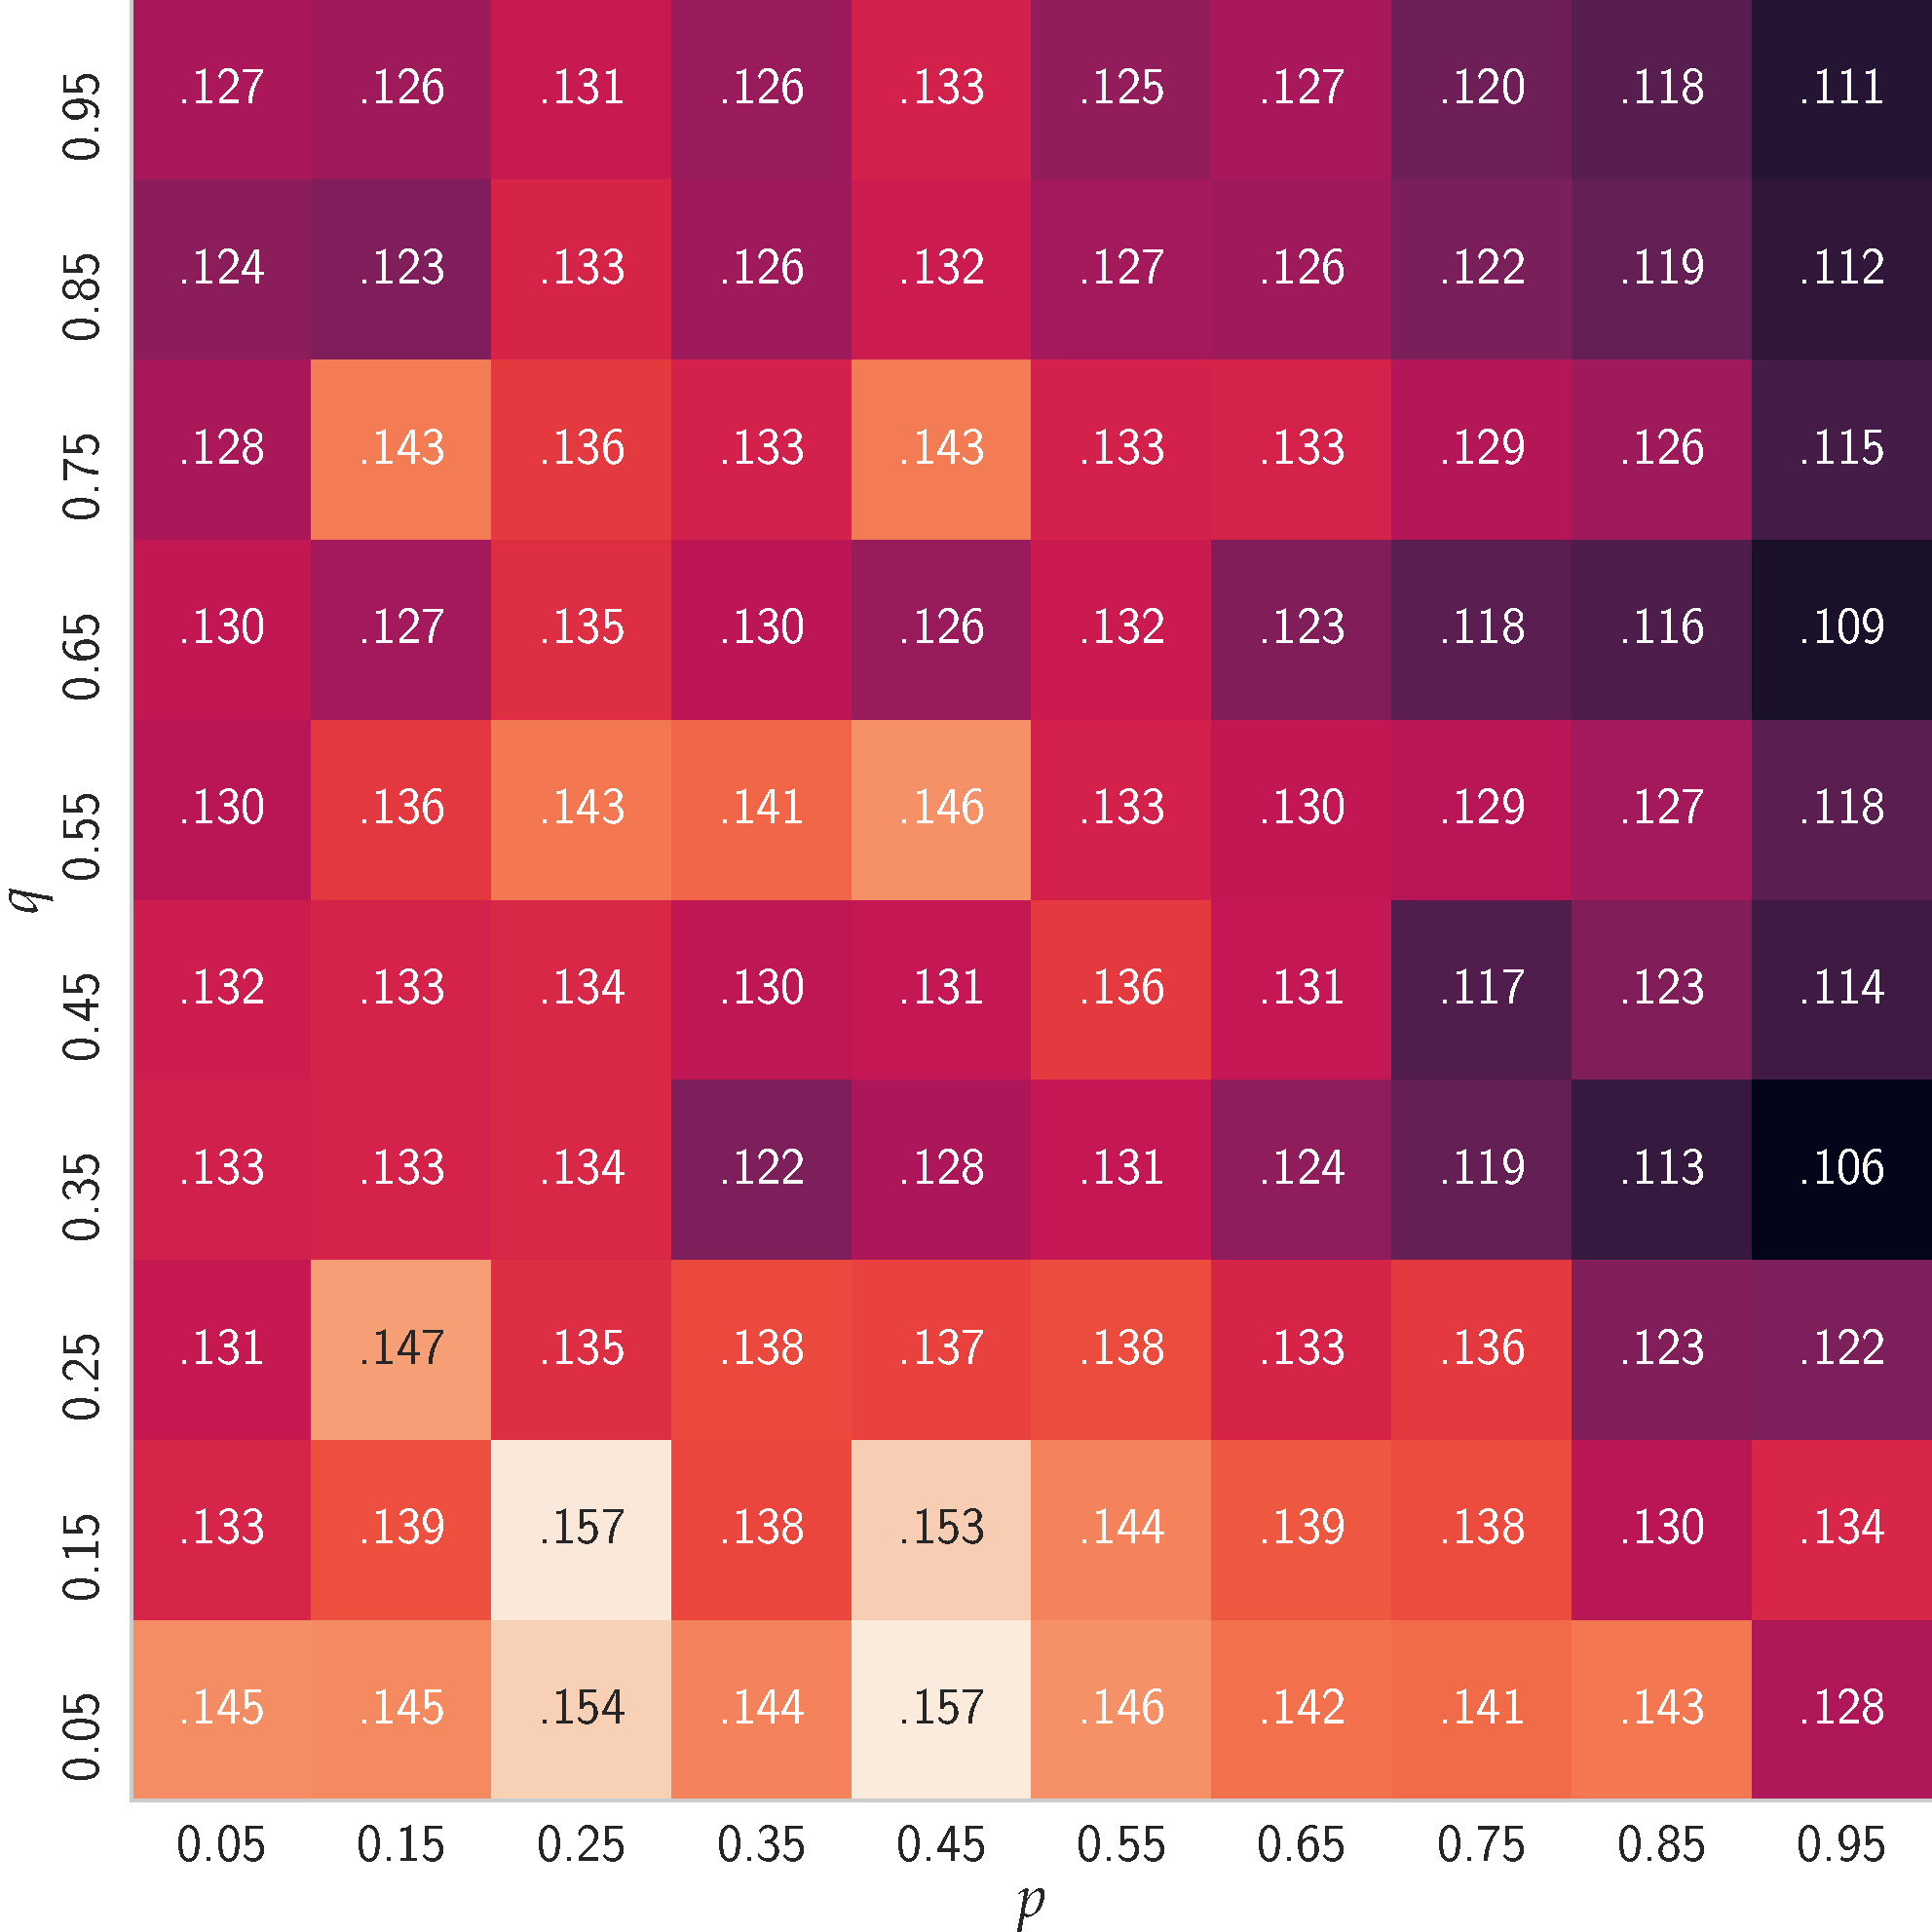
\includegraphics[width=\textwidth]{raw/synthgen_wik_rule_40_mae.pdf} 
    \caption{Mean absolute error (MAE) of the \etauv{} estimation.} 
    \label{fig:tr_synth_mae}
  \end{subfigure}~
  \begin{subfigure}[b]{0.504\textwidth} 
    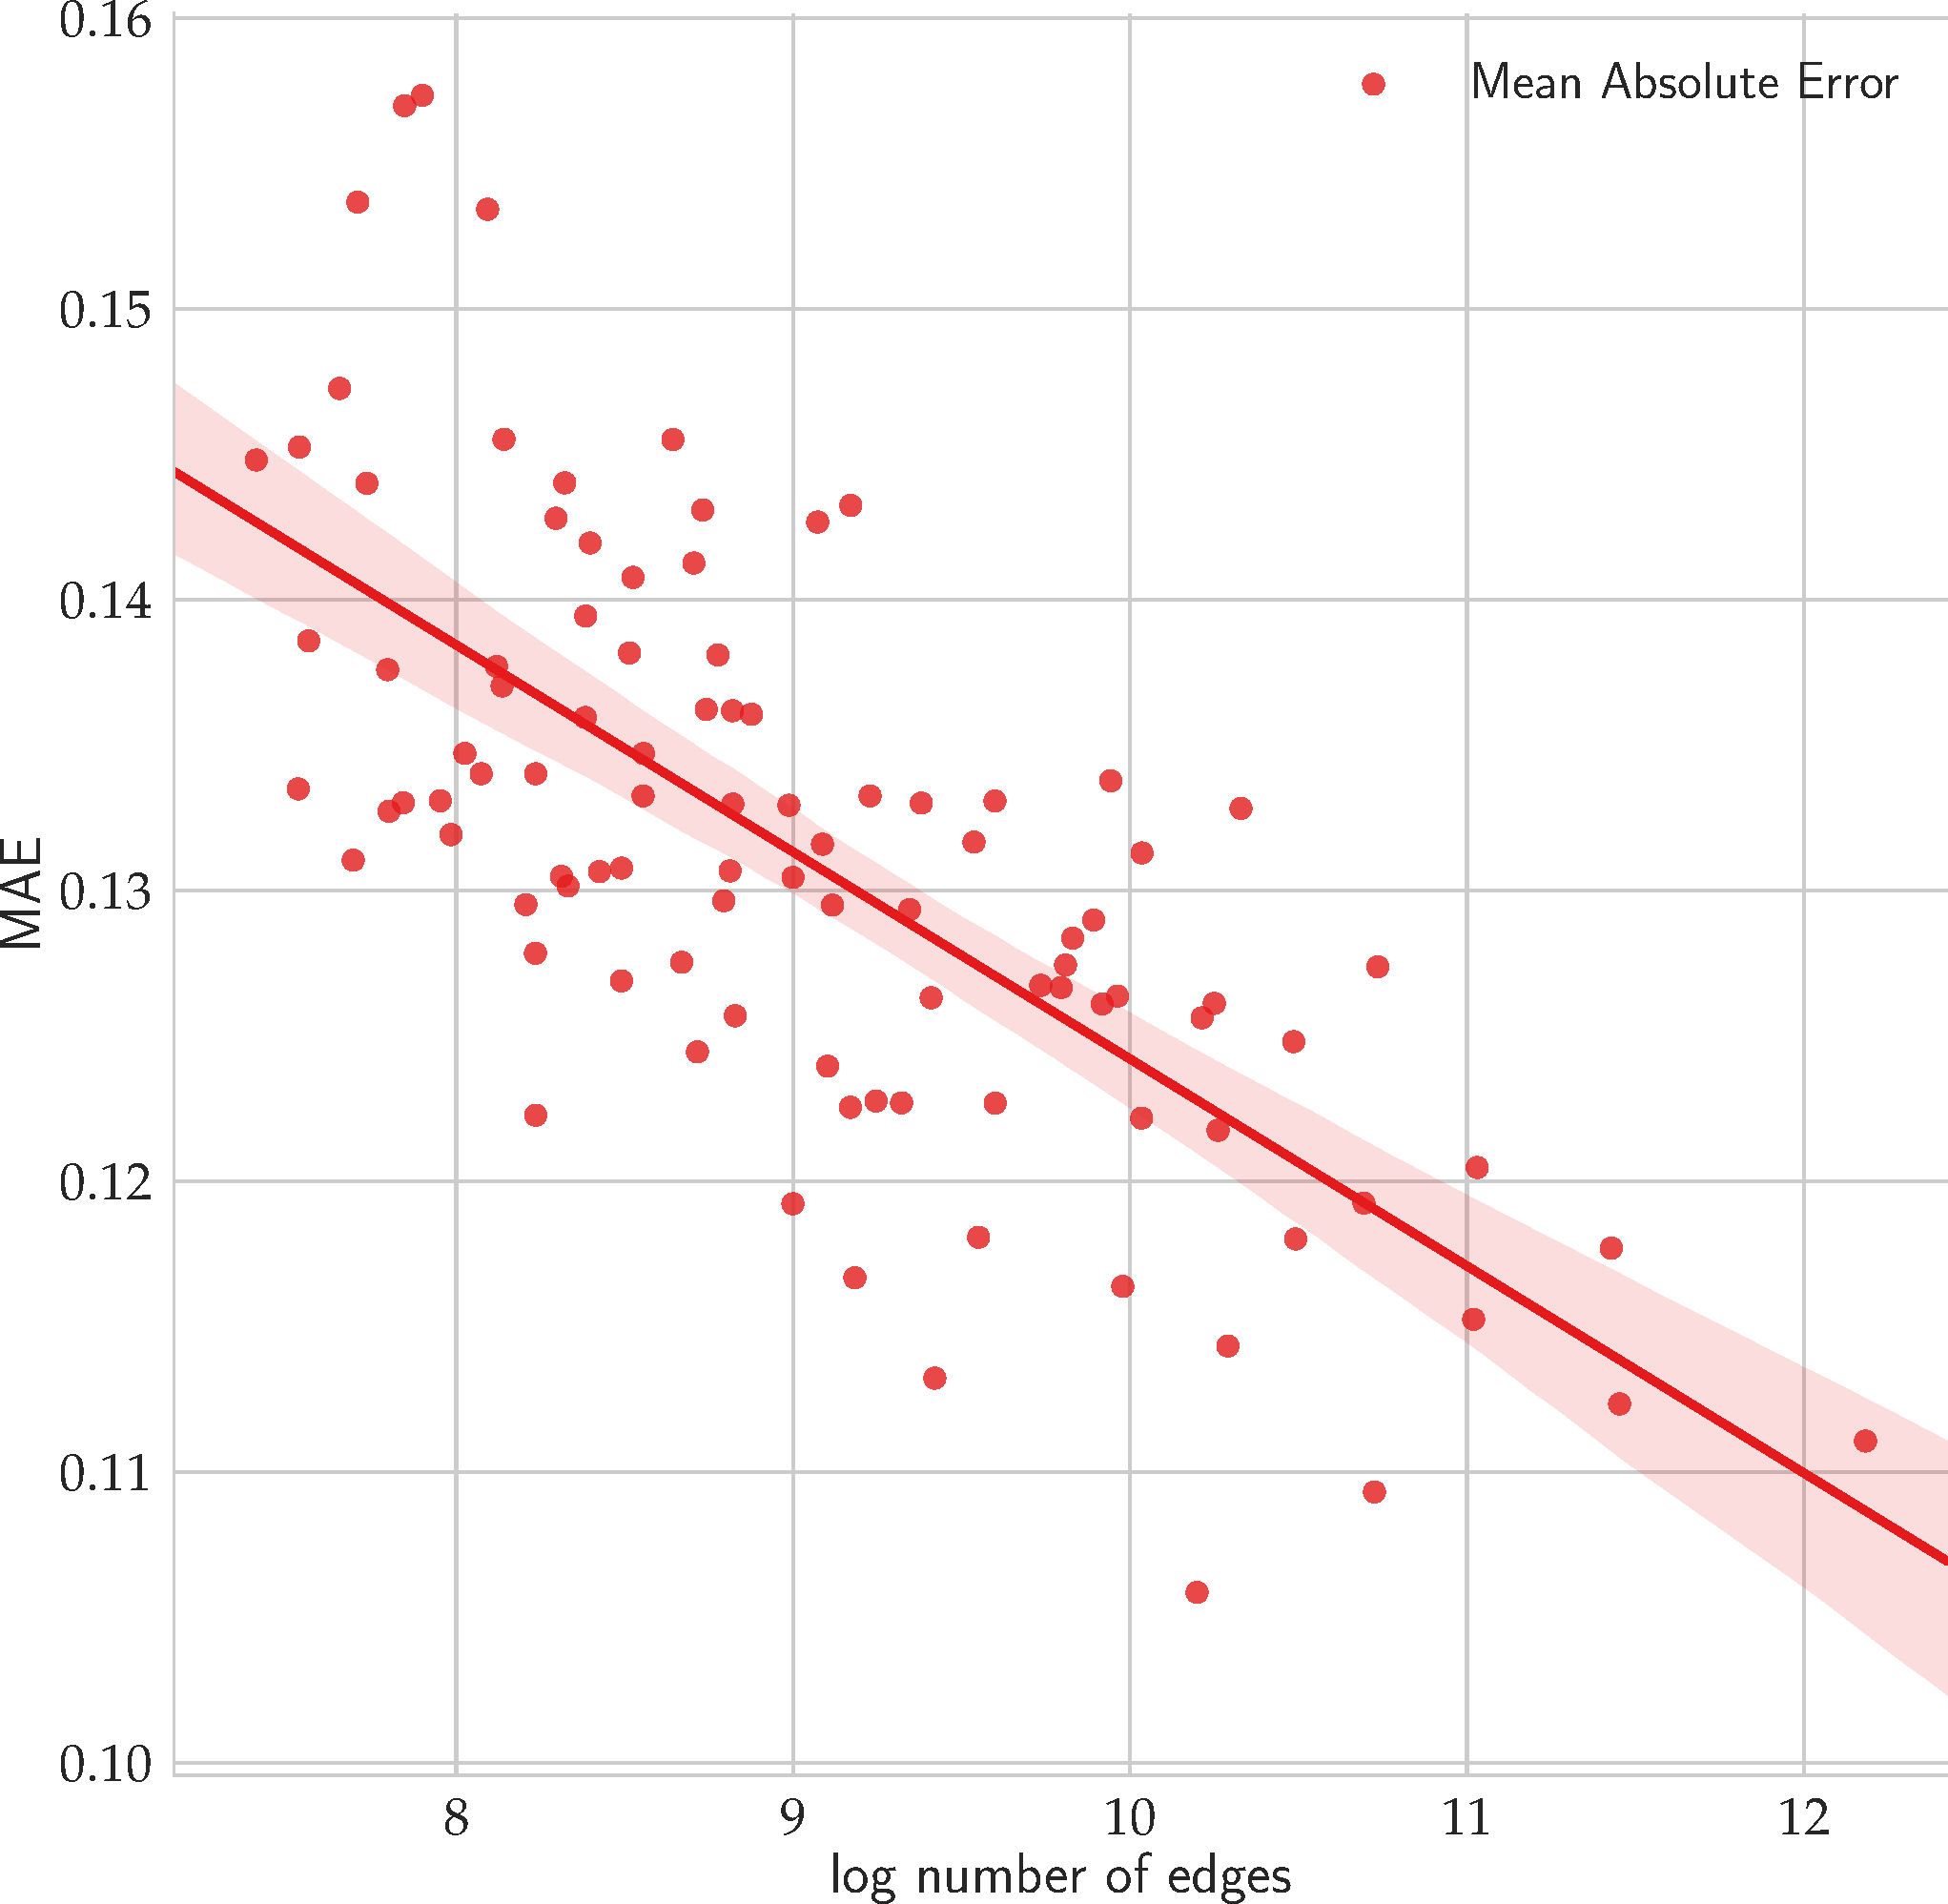
\includegraphics[width=\textwidth]{raw/synthgen_wik_rule_40_sizemae.pdf} 
    \caption{MAE in each cell as a function of the number of sampled edges.} 
    \label{fig:tr_synth_sizemae}
  \end{subfigure}

  \begin{subfigure}[b]{0.504\textwidth} 
    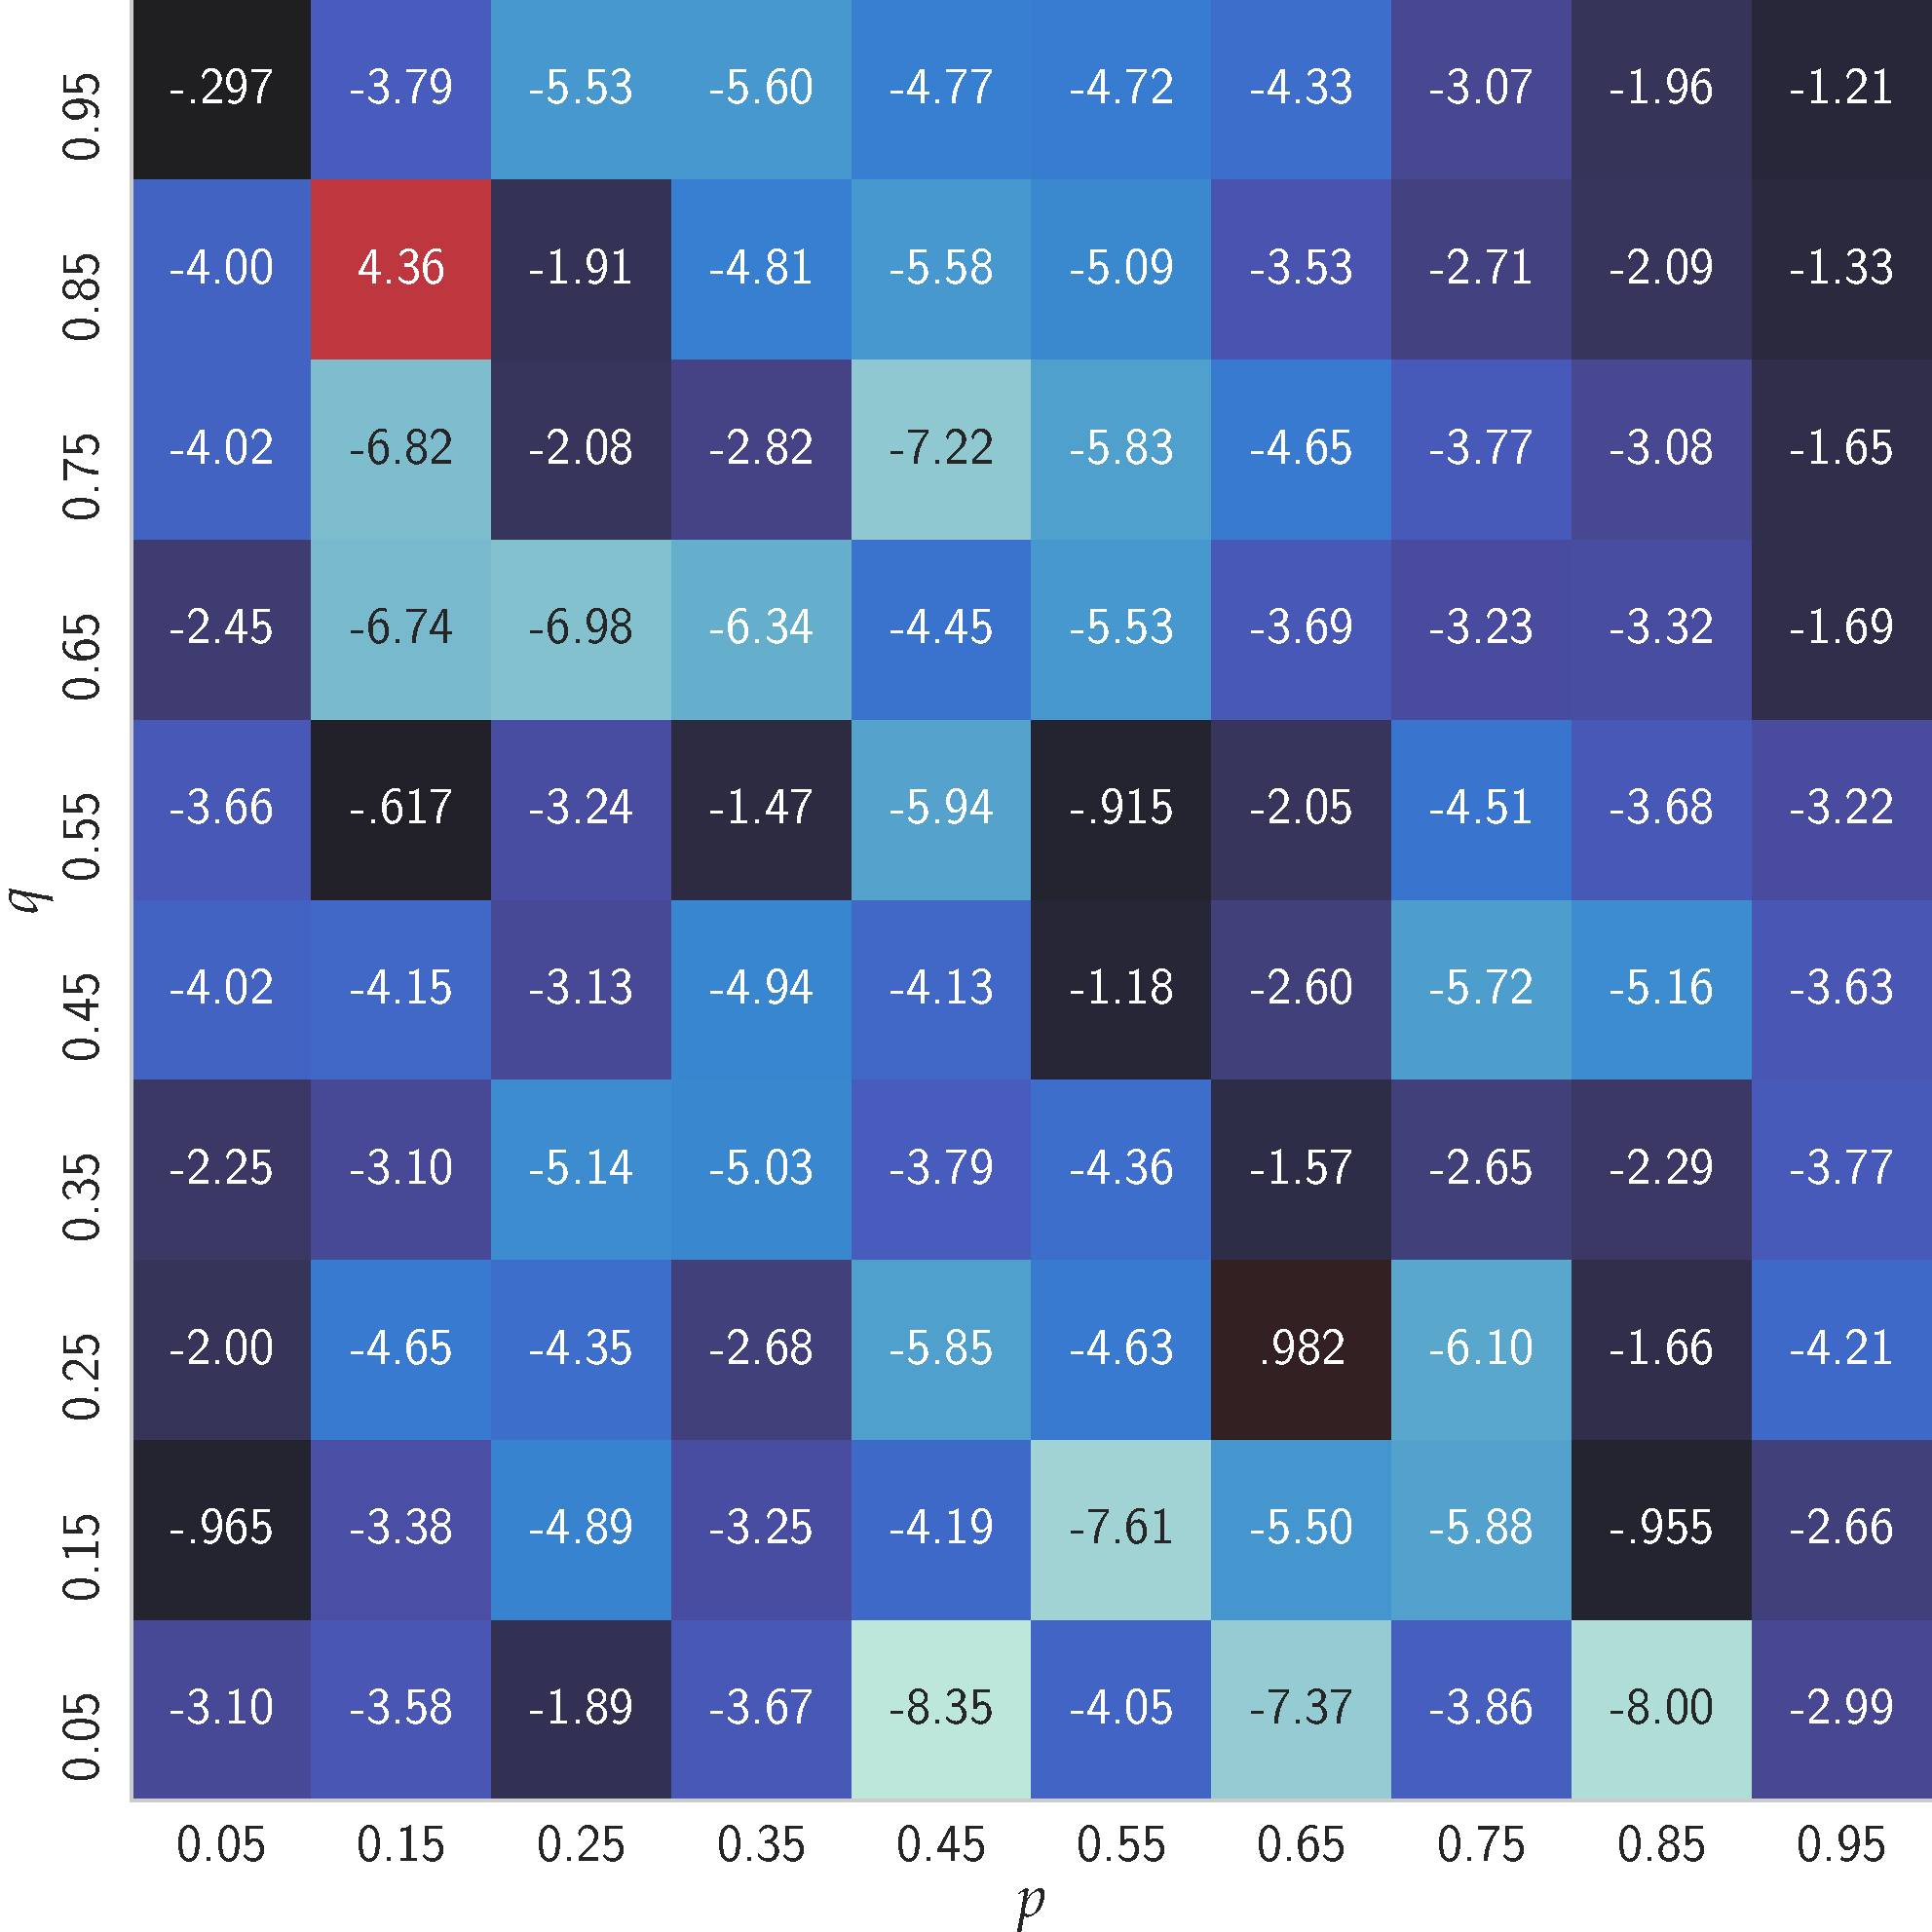
\includegraphics[width=\textwidth]{raw/synthgen_wik_rule_40_acc.pdf} 
    \caption{100 time the difference of accuracy between \usrule{} and Bayes.} 
    \label{fig:tr_synth_acc}
  \end{subfigure}~
  \begin{subfigure}[b]{0.504\textwidth} 
    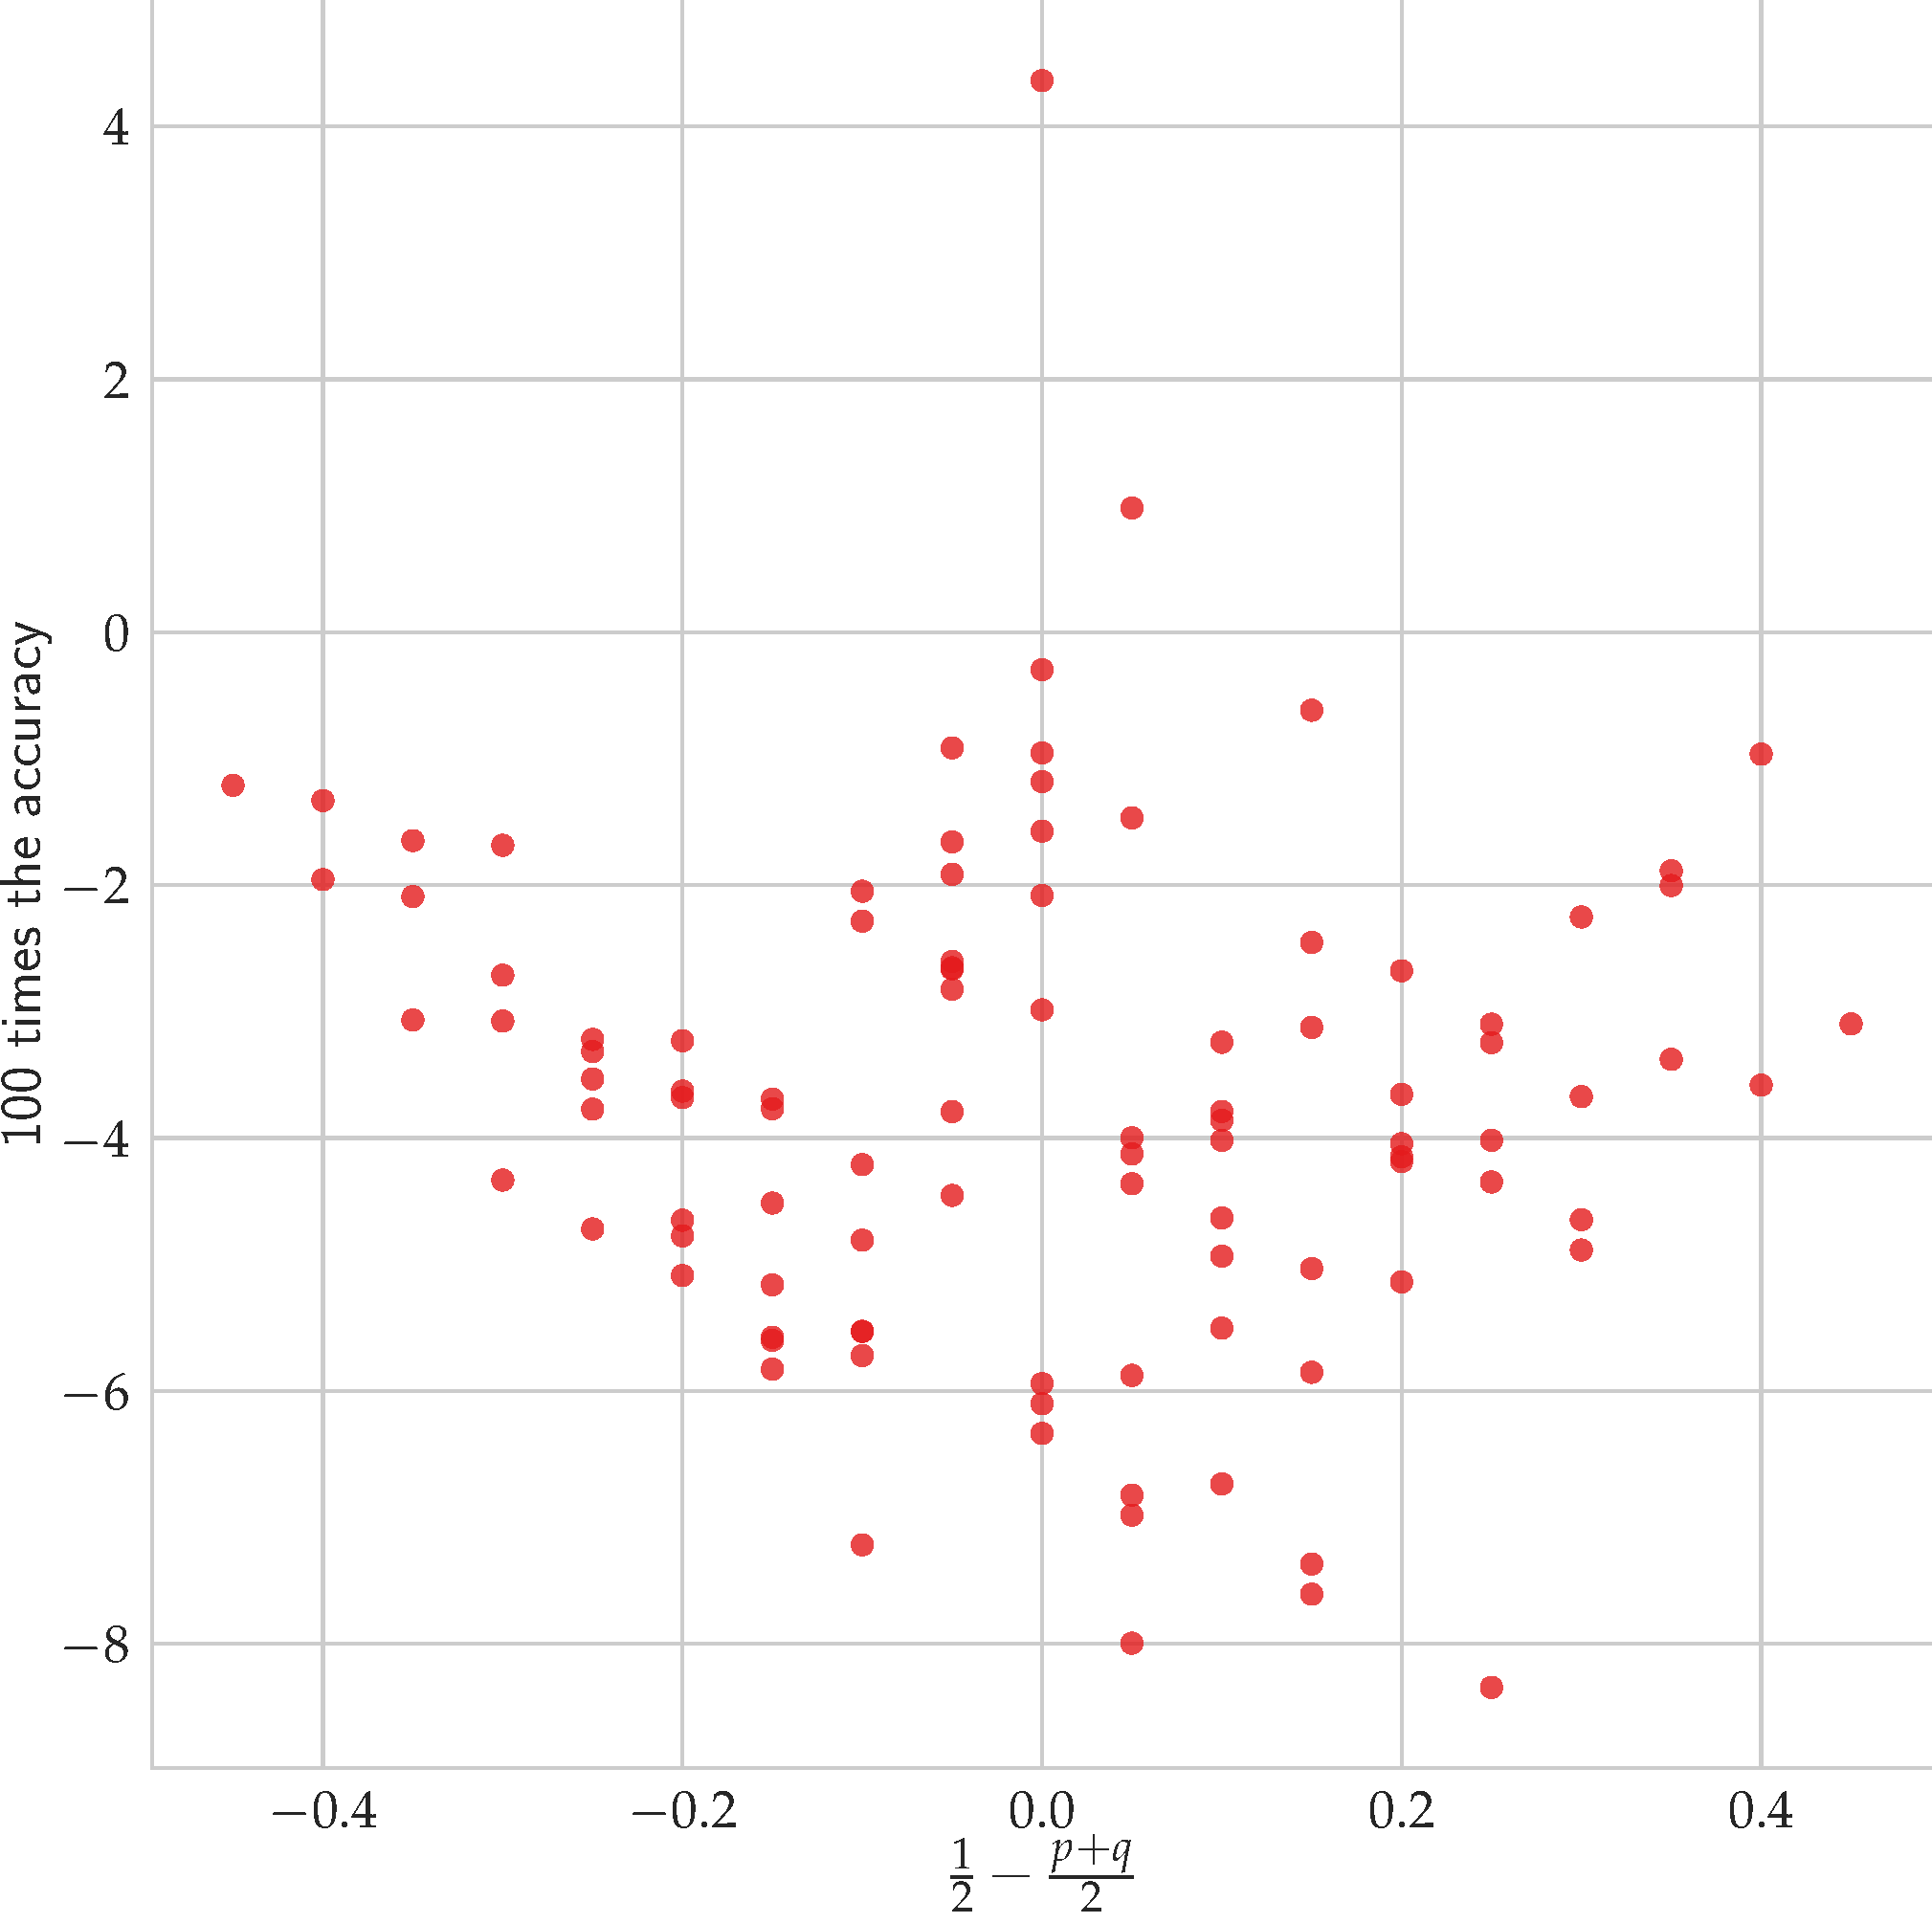
\includegraphics[width=\textwidth]{raw/synthgen_wik_rule_40_cmpacc.pdf} 
    \caption{Difference of accuracy between \usrule{} and Bayes as $\frac{p+q}{2}$ moves away from $\frac{1}{2}$.} 
    \label{fig:tr_synth_cmpacc}
  \end{subfigure}
  \caption{Results on \wik{} with \usrule{} on a training set of size 40\%}
\end{figure*}

\subsection{Real signs} 
We compared the following algorithms:

\begin{enumerate}[label=\textbf{\arabic*.}]
  \item The label propagation algorithm of \autoref{ss:passive} (referred to as \uslpropGsec{}).
    The actual binarizing threshold was set by cross-validation on the training set.

  \item The \usrule{} algorithm described in \autoref{ss:passive}.

  \item A logistic regression model where each edge $(u,v)$ is associated with the features
    $[1-\htr(u), 1-\hun(v)]$ computed again on \trainset{} (we call this method \uslogregp{}). The best
    binary thresholding is again computed on \trainset{}. Experimenting with this logistic model
    serves to support the claim we made in the introduction that our generative model in
    \autoref{s:gen} is a good fit for the data.

  \item  The solution obtained by directly solving the unregularized problem \eqref{e:quadratic}
    through a fast constrained minimization algorithm (referred to as \qoptim{}). Again, the actual
    binarizing threshold was set by cross-validation on the training set.\footnote{We have also
    tried to minimize \eqref{e:quadratic} by removing the $[-1,+1]$ constraints, but got similar MCC
    results as the ones we report for \qoptim{}}

  \item  The matrix completion method from~\autocite{LowRankCompletion14} based on \complowrank{}
    matrix factorization. Since the authors showed their method to be robust to the choice of the
    rank parameter $k$, we picked $k=7$ in our experiments.

  \item The other \compmaxnorm{} matrix completion method from~\autocite{OnlineCompletion17},
    setting the parameter $\lambda$ to $1.2$ as advised in their paper.

  \item A logistic regression model built on \comptriads{} features derived from status
    theory~\autocite{Leskovec2010}.

  \item The TrollTrust algorithm from~\autocite{wu2016troll}, naming it \compranknodes{}. As for
    hyperparameter tuning ($\beta$ and $\lambda_1$ in~\autocite{wu2016troll}), we closely followed
    the authors' suggestion of doing cross validation.

  \item  The last competitor is the logistic regression model whose features have been build
    according to \autocite{Bayesian15}. We call this method \compbayesian{}.
\end{enumerate}

The above methods can be roughly divided into \emph{local} and \emph{global} methods. A local method
hinges on building local predictive features, based on neighborhoods: \usrule{}, \uslogregp{},
\comptriads{}, and \compbayesian{} essentially fall into this category. The remaining methods
(\uslpropGsec{}, \complowrank{}, \compmaxnorm{} and \compranknodes{}) are global in that their
features are
designed to depend on global properties of the graph topology.

\iffalse
%Given a training set \trainset{}, we exploit the revealed signs in two ways.
First, with label propagation (referred to as \uslprop{} in the following). We
initialize the labels vector $f_0$ to $|V'|$ random values drawn uniformly in
$[0, 1]$ and set the label of the training edges equal to their observed value.
% TODO: starting with zeros gives lower MCC and accuracy after a fixed number
% of iterations
Let the adjacency matrix of $G'$ be $A$, its diagonal degree matrix
be $D$, its diameter be $\diam{G'}$ and $P$ be the following sparse matrix $P=D^{-1}A$. This allow performing
one round of label propagation as $f_{t+1} = Pf_t$, followed by clamping the
training labels. Each round thus involves $2|E|$ multiplications and we do
$\diam{G'}$ of them\footnote{$\diam{G'}$ is a small constant, ranging from $16$
for \aut{} to $38$ for \epi{}}. With the computed labels, we can associate each
edge $\eij$ with $a_{i,j} = \nicefrac{1}{2}\left(f_{\diam{G'}}(\iout) +
f_{\diam{G'}}(\jin)\right)$.
% This is what I do in the code but now I realize this is just an extra
% propagation round only on the square node so maybe simplify the description
% (actually no, it's needed for ERM)
By sorting the $a$ values of the training edges, we can find the threshold $t$
that minimizes the number of mistakes on the training set while predicting
$\yij = \sgn\left(a_{i,j} - t\right)$ in $O(|\trainset{}|\log |\trainset{}|)$
time.

Then we again associate each edge $\eij$ with $a_{i,j} = \left(1-\htr(i)\right) +
\left(1-\hun(j)\right)$ and find the $\tau$ of \eqref{eq:predictor} that minimizes the empirical
risk.  Another way to exploit those quantities is to train a Logistic Regression model where each
edge is associated with two features: $[1-\htr(i), 1-\hun(j)]$ (we call this method \uslogregp{}).
\fi

\bigskip

Our main results are summarized in \autoref{tab:all_mcc}, reporting MCC test set performance after
training on sets of varying size (from 5\% to 25\%, plus 50\% and 90\%). Results have been averaged
over 12 repetitions.
Because scalability is a major concern when training on sizeable datasets, we also give an idea of
relative training times (in milliseconds) by reporting separately in \autoref{tab:all_time} the time it took to train a single run of
each algorithm on a training set of size\footnote{Comparison of training time performances is fair
since all algorithms have been carefully implemented using the same stack of Python libraries, and
run on the same machine (16 Xeon cores and 192Gb Ram).} 15\% of $|E|$, and then predict on the test
set. Some conclusions emerge from those experiments:


\begin{enumerate}[leftmargin=2em,label=\textbf{\arabic*.}]

  \item Global methods tend to outperform local methods in terms of prediction performance, but are
    also significantly (or even much) slower (running times can differ by as much as three orders of
    magnitude). This is not surprising, and is in line with previous experimental findings (e.g.,
    \autocites{shahriari2014ranking}{wu2016troll}). \compbayesian{} looks like an exception to this
    rule, but its running time is indeed in the same ballpark as global methods.

  \item \uslpropGsec{} almost always ranks first or at least second in this comparison when MCC is
    considered, at least in the small training set regime (that is when having access to at most
    $25\%$ of the labels, which might be more realistic in many real world situations).
    On top of it, \uslpropGsec{} is fastest among the global methods (one or even two
    orders of magnitude faster), thereby showing the benefit of our approach to \esp{}.

  \item Two methods are competitive with us, \compbayesian{} and \compranknodes{}. \compbayesian{}
    achieves its best results on the larger dataset (\sla{}, \epi{} and \kiw{}) when the training
    set size is large. Indeed, it learns a much more complex model than our methods, with $256$
    parameters\footnote{corresponding to $16\times 16$ feature per edge}, which also requires a lot
    of time to be trained. \compranknodes{} also shines in those large datasets, even at small
    training size. Note however that the difference with \uslpropGsec{} is usually less than one point,
    at the expense of a five times longer learning time.

  \item The regularized solution computed by \uslpropGsec{} is always better than the unregularized
    one computed by \qoptim{} in terms of both MCC and running time.

  \item As claimed in the introduction, our Bayes approximator \usrule{} closely mirrors in
    performance the more involved \uslogregp{} model. In fact, supporting our generative model of
    \autoref{s:gen}, the logistic regression weights for features $1-\htr(i)$ and $1-\hun(j)$
    are almost equal (see \autoref{tab:coeff} in the supplementary material), thereby suggesting that
    predictor~\eqref{eq:predictor}, derived from the theoretical results in
    \autoref{ss:bayes_approx}, is \emph{also} the best logistic model based on trollness and
    untrustworthiness.
\end{enumerate}

% \begin{table}[tbp]
%   \centering
\begingroup
  \setlength{\tabcolsep}{3pt}
  \scriptsize
  \setlength\LTleft{ -1cm}
  \setlength\LTright{-1cm}
  \begin{longtable}{lrcccc|ccccc}
  \caption{MCC with increasing training set size, with one standard deviation over 12 random sampling of
    $\trainset$. The last five columns refer to the methods we took from the literature. For the sake of
    readability, we multiplied all MCC values by 100. The best number in each row is highlighted in
    \textbf{\textcolor{brown}{bold brown}} and the second one in \textit{\textcolor{red}{italic red}}.
    If the difference is statistically significant ($p$-value of a paired Student's $t$-test less than
    $0.005$), the best score is underlined.
  \label{tab:all_mcc}}\\
  % \begin{tabular}{lrcccc|ccccc}
    \toprule
                                                      & $\frac{|\trainset{}|}{|E|}$ & \uslpropGsec{}              & \usrule{}                   & \uslogregp{}                & \usoptim{}                  & \complowrank{} & \compmaxnorm{}             & \comptriads{}  & \compranknodes{}            & \compbayesian{}             \\
    \midrule
    \endfirsthead
    \toprule
                                                      & $\frac{|\trainset{}|}{|E|}$ & \uslpropGsec{}              & \usrule{}                   & \uslogregp{}                & \usoptim{}                  & \complowrank{} & \compmaxnorm{}             & \comptriads{}  & \compranknodes{}            & \compbayesian{}             \\
    \midrule
    \endhead
\multirow{9}{*}{\rotatebox[origin=c]{90}{\aut{}}} & $5\%$  &  $\vfirstSig{24.2} \pm 0.9$  &  $\vsecondSig{19.8} \pm 0.5$  &               $19.8 \pm 0.5$  &  $15.9 \pm 0.5$  &  $12.4 \pm 0.7$  &               $1.2 \pm 1.4$  &  $11.4 \pm 1.1$  &  $17.5 \pm 1.0$  &               $15.2 \pm 1.4$  \\
                                                  & $10\%$ &  $\vfirstSig{31.7} \pm 0.8$  &  $\vsecondSig{28.0} \pm 0.6$  &               $27.9 \pm 0.7$  &  $26.0 \pm 0.7$  &  $17.9 \pm 0.7$  &              $12.6 \pm 0.8$  &  $17.2 \pm 1.0$  &  $25.1 \pm 0.9$  &               $25.5 \pm 0.9$  \\
                                                  & $15\%$ &  $\vfirstSig{36.1} \pm 0.7$  &               $33.1 \pm 0.8$  &  $\vsecondSig{33.2} \pm 0.7$  &  $31.6 \pm 0.7$  &  $22.0 \pm 0.6$  &              $22.2 \pm 0.9$  &  $21.0 \pm 1.0$  &  $31.2 \pm 1.0$  &               $32.0 \pm 0.8$  \\
                                                  & $20\%$ &  $\vfirstSig{38.9} \pm 0.8$  &  $\vsecondSig{37.1} \pm 0.6$  &               $36.9 \pm 0.6$  &  $35.6 \pm 0.5$  &  $25.7 \pm 0.9$  &              $30.3 \pm 0.8$  &  $24.3 \pm 0.7$  &  $35.2 \pm 0.7$  &               $36.7 \pm 0.5$  \\
                                                  & $25\%$ &  $\vfirstSig{41.1} \pm 0.7$  &               $39.7 \pm 0.8$  &               $39.7 \pm 0.7$  &  $38.4 \pm 0.9$  &  $29.0 \pm 0.6$  &              $36.5 \pm 0.9$  &  $27.0 \pm 0.6$  &  $37.8 \pm 0.9$  &  $\vsecondSig{39.8} \pm 1.0$  \\
                                                  & $50\%$ &              $47.2 \pm 0.6$  &               $48.1 \pm 0.6$  &               $47.7 \pm 0.5$  &  $46.7 \pm 0.7$  &  $44.9 \pm 1.4$  &  $\vfirstSig{55.9} \pm 0.9$  &  $35.4 \pm 1.0$  &  $46.0 \pm 0.6$  &  $\vsecondSig{50.9} \pm 0.8$  \\
                                                  & $90\%$ &              $51.6 \pm 2.1$  &               $52.6 \pm 2.2$  &               $52.5 \pm 1.7$  &  $52.3 \pm 1.9$  &  $60.4 \pm 1.6$  &  $\vfirstSig{66.7} \pm 1.0$  &  $47.2 \pm 1.9$  &  $51.5 \pm 2.1$  &  $\vsecondSig{61.7} \pm 1.3$  \\
\midrule
\multirow{9}{*}{\rotatebox[origin=c]{90}{\adv{}}} & $5\%$  &   $\vfirstSig{40.9} \pm 0.7$  &  $36.5 \pm 0.7$  &  $\vsecondSig{36.8} \pm 0.8$  &               $30.2 \pm 0.8$  &  $25.1 \pm 1.0$  &   $4.7 \pm 3.3$  &  $29.5 \pm 3.7$  &  $32.2 \pm 1.0$  &  $19.8 \pm 0.8$  \\
                                                  & $10\%$ &   $\vfirstSig{46.8} \pm 0.6$  &  $44.7 \pm 0.6$  &  $\vsecondSig{45.3} \pm 0.7$  &               $42.8 \pm 0.9$  &  $28.3 \pm 0.7$  &  $24.2 \pm 1.6$  &  $37.6 \pm 1.4$  &  $38.8 \pm 1.0$  &  $30.7 \pm 0.9$  \\
                                                  & $15\%$ &     $\vsecond{50.4} \pm 0.5$  &  $49.5 \pm 0.6$  &      $\vfirst{50.4} \pm 0.6$  &               $47.9 \pm 0.6$  &  $30.3 \pm 0.8$  &  $30.1 \pm 1.1$  &  $42.0 \pm 0.8$  &  $45.1 \pm 1.6$  &  $38.5 \pm 0.8$  \\
                                                  & $20\%$ &  $\vsecondSig{52.2} \pm 0.6$  &  $51.9 \pm 0.5$  &   $\vfirstSig{53.0} \pm 0.5$  &               $51.1 \pm 0.7$  &  $31.5 \pm 0.7$  &  $33.5 \pm 1.3$  &  $44.4 \pm 0.6$  &  $48.9 \pm 0.9$  &  $43.4 \pm 0.6$  \\
                                                  & $25\%$ &  $\vsecondSig{54.2} \pm 0.7$  &  $54.1 \pm 0.5$  &   $\vfirstSig{55.3} \pm 0.5$  &               $53.7 \pm 0.6$  &  $32.7 \pm 0.7$  &  $35.6 \pm 1.1$  &  $46.7 \pm 0.9$  &  $51.7 \pm 1.1$  &  $47.6 \pm 0.7$  \\
                                                  & $50\%$ &               $59.0 \pm 0.5$  &  $59.8 \pm 0.5$  &   $\vfirstSig{60.7} \pm 0.4$  &  $\vsecondSig{60.3} \pm 0.4$  &  $37.1 \pm 0.8$  &  $42.8 \pm 1.2$  &  $52.2 \pm 0.9$  &  $58.2 \pm 0.6$  &  $56.5 \pm 0.5$  \\
                                                  & $90\%$ &               $63.3 \pm 1.3$  &  $64.0 \pm 1.2$  &     $\vsecond{64.5} \pm 1.2$  &      $\vfirst{65.0} \pm 1.1$  &  $44.0 \pm 2.0$  &  $49.5 \pm 1.9$  &  $57.9 \pm 1.3$  &  $63.3 \pm 1.1$  &  $63.0 \pm 1.2$  \\
\midrule
\multirow{9}{*}{\rotatebox[origin=c]{90}{\wik{}}} & $5\%$  &  $\vfirstSig{39.8} \pm 0.7$  &  $38.2 \pm 1.0$  &  $\vsecondSig{39.0} \pm 0.7$  &  $36.0 \pm 0.7$  &  $24.7 \pm 0.8$  &  $24.6 \pm 0.9$  &   $9.7 \pm 1.0$  &            $33.4 \pm 0.6$  &  $26.2 \pm 1.4$  \\
                                                  & $10\%$ &    $\vsecond{46.7} \pm 0.6$  &  $45.9 \pm 0.5$  &      $\vfirst{46.8} \pm 0.5$  &  $44.4 \pm 0.6$  &  $31.5 \pm 0.7$  &  $34.9 \pm 0.4$  &  $26.8 \pm 1.5$  &            $43.2 \pm 0.6$  &  $40.3 \pm 0.6$  \\
                                                  & $15\%$ &    $\vsecond{50.3} \pm 0.5$  &  $49.6 \pm 0.4$  &      $\vfirst{50.5} \pm 0.4$  &  $48.8 \pm 0.4$  &  $35.4 \pm 0.7$  &  $39.4 \pm 0.6$  &  $34.2 \pm 0.6$  &            $48.4 \pm 0.5$  &  $46.7 \pm 0.4$  \\
                                                  & $20\%$ &    $\vsecond{52.5} \pm 0.4$  &  $51.9 \pm 0.5$  &      $\vfirst{52.8} \pm 0.5$  &  $51.7 \pm 0.5$  &  $38.0 \pm 0.6$  &  $42.2 \pm 0.5$  &  $38.2 \pm 0.7$  &            $51.2 \pm 0.5$  &  $50.2 \pm 0.4$  \\
                                                  & $25\%$ &    $\vsecond{54.2} \pm 0.6$  &  $53.6 \pm 0.6$  &      $\vfirst{54.6} \pm 0.5$  &  $53.6 \pm 0.4$  &  $40.2 \pm 0.6$  &  $44.2 \pm 0.6$  &  $41.2 \pm 0.6$  &            $53.5 \pm 0.5$  &  $53.0 \pm 0.6$  \\
                                                  & $50\%$ &    $\vsecond{57.8} \pm 0.3$  &  $56.9 \pm 0.5$  &      $\vfirst{57.9} \pm 0.4$  &  $57.6 \pm 0.4$  &  $47.3 \pm 0.7$  &  $48.8 \pm 0.7$  &  $48.9 \pm 0.5$  &            $57.8 \pm 0.4$  &  $57.4 \pm 0.5$  \\
                                                  & $90\%$ &     $\vfirst{60.5} \pm 0.8$  &  $59.5 \pm 0.9$  &               $60.4 \pm 0.9$  &  $59.9 \pm 1.1$  &  $53.5 \pm 0.9$  &  $51.3 \pm 0.8$  &  $55.6 \pm 0.8$  &  $\vsecond{60.4} \pm 1.0$  &  $59.6 \pm 1.2$  \\
\midrule
\multirow{9}{*}{\rotatebox[origin=c]{90}{\sla{}}} & $5\%$  &  $\vsecondSig{41.0} \pm 0.2$  &  $36.3 \pm 0.5$  &  $37.1 \pm 0.3$  &  $33.6 \pm 0.2$  &  $36.9 \pm 0.4$  &  $14.9 \pm 0.8$  &  $27.8 \pm 1.0$  &   $\vfirstSig{45.3} \pm 0.4$  &              $29.4 \pm 0.3$  \\
                                                  & $10\%$ &  $\vsecondSig{46.6} \pm 0.2$  &  $42.2 \pm 0.2$  &  $43.1 \pm 0.2$  &  $40.9 \pm 0.3$  &  $39.7 \pm 0.3$  &  $25.7 \pm 0.7$  &  $40.3 \pm 1.1$  &   $\vfirstSig{47.8} \pm 0.5$  &              $38.2 \pm 0.2$  \\
                                                  & $15\%$ &   $\vfirstSig{49.7} \pm 0.2$  &  $45.4 \pm 0.3$  &  $46.5 \pm 0.2$  &  $45.4 \pm 0.2$  &  $41.3 \pm 0.3$  &  $32.5 \pm 0.3$  &  $45.5 \pm 1.3$  &  $\vsecondSig{48.7} \pm 0.7$  &              $43.4 \pm 0.2$  \\
                                                  & $20\%$ &     $\vsecond{51.8} \pm 0.2$  &  $47.6 \pm 0.3$  &  $48.7 \pm 0.1$  &  $48.3 \pm 0.2$  &  $42.9 \pm 0.2$  &  $36.6 \pm 0.3$  &  $49.0 \pm 0.7$  &      $\vfirst{52.0} \pm 0.3$  &              $47.0 \pm 0.3$  \\
                                                  & $25\%$ &     $\vsecond{53.3} \pm 0.2$  &  $49.4 \pm 0.2$  &  $50.2 \pm 0.1$  &  $50.0 \pm 0.1$  &  $44.3 \pm 0.6$  &  $39.7 \pm 0.3$  &  $50.6 \pm 0.4$  &      $\vfirst{53.3} \pm 0.3$  &              $49.4 \pm 0.2$  \\
                                                  & $50\%$ &   $\vfirstSig{57.2} \pm 0.1$  &  $54.2 \pm 0.2$  &  $55.0 \pm 0.1$  &  $54.6 \pm 0.1$  &  $52.9 \pm 0.5$  &  $48.2 \pm 0.1$  &  $55.2 \pm 0.4$  &  $\vsecondSig{56.8} \pm 0.2$  &              $56.3 \pm 0.1$  \\
                                                  & $90\%$ &  $\vsecondSig{59.6} \pm 0.5$  &  $57.4 \pm 0.5$  &  $58.0 \pm 0.5$  &  $57.7 \pm 0.4$  &  $59.0 \pm 0.4$  &  $53.5 \pm 0.4$  &  $58.0 \pm 0.4$  &               $59.2 \pm 0.6$  &  $\vfirstSig{61.1} \pm 0.5$  \\
\midrule
\multirow{9}{*}{\rotatebox[origin=c]{90}{\epi{}}} & $5\%$  &  $\vsecondSig{54.6} \pm 0.3$  &  $46.9 \pm 0.6$  &  $48.9 \pm 0.3$  &  $42.8 \pm 0.4$  &  $39.9 \pm 0.3$  &  $28.9 \pm 0.3$  &  $41.4 \pm 2.0$  &   $\vfirstSig{56.0} \pm 0.6$  &              $37.9 \pm 0.4$  \\
                                                  & $10\%$ &  $\vsecondSig{59.0} \pm 0.4$  &  $54.1 \pm 0.4$  &  $55.9 \pm 0.2$  &  $53.3 \pm 0.4$  &  $44.4 \pm 0.3$  &  $36.7 \pm 0.4$  &  $50.8 \pm 1.5$  &   $\vfirstSig{60.5} \pm 0.3$  &              $49.9 \pm 0.4$  \\
                                                  & $15\%$ &  $\vsecondSig{61.5} \pm 0.3$  &  $57.9 \pm 0.3$  &  $59.3 \pm 0.1$  &  $58.7 \pm 0.5$  &  $48.6 \pm 0.7$  &  $41.0 \pm 0.5$  &  $54.5 \pm 1.8$  &   $\vfirstSig{62.7} \pm 0.2$  &              $56.5 \pm 0.7$  \\
                                                  & $20\%$ &  $\vsecondSig{63.0} \pm 0.3$  &  $60.3 \pm 0.3$  &  $61.4 \pm 0.1$  &  $61.8 \pm 0.2$  &  $52.0 \pm 0.9$  &  $43.9 \pm 0.4$  &  $56.3 \pm 1.2$  &   $\vfirstSig{64.1} \pm 0.3$  &              $61.4 \pm 0.4$  \\
                                                  & $25\%$ &               $64.2 \pm 0.2$  &  $61.8 \pm 0.3$  &  $62.9 \pm 0.1$  &  $63.5 \pm 0.1$  &  $55.0 \pm 0.7$  &  $46.3 \pm 0.4$  &  $58.6 \pm 1.4$  &      $\vfirst{65.2} \pm 0.6$  &    $\vsecond{64.7} \pm 0.3$  \\
                                                  & $50\%$ &               $67.3 \pm 0.2$  &  $66.3 \pm 0.2$  &  $66.7 \pm 0.1$  &  $67.2 \pm 0.2$  &  $63.4 \pm 0.3$  &  $52.8 \pm 0.2$  &  $64.2 \pm 1.4$  &  $\vsecondSig{69.9} \pm 0.2$  &  $\vfirstSig{72.5} \pm 0.1$  \\
                                                  & $90\%$ &               $69.7 \pm 0.3$  &  $69.2 \pm 0.3$  &  $69.1 \pm 0.3$  &  $69.7 \pm 0.3$  &  $68.0 \pm 0.7$  &  $57.6 \pm 0.6$  &  $67.6 \pm 0.7$  &  $\vsecondSig{71.6} \pm 0.3$  &  $\vfirstSig{77.4} \pm 0.4$  \\
\midrule
\multirow{9}{*}{\rotatebox[origin=c]{90}{\kiw{}}} & $5\%$  &   $\vfirstSig{36.5} \pm 0.4$  &  $\vsecondSig{31.0} \pm 0.2$  &               $30.8 \pm 0.2$  &  $21.9 \pm 0.3$  &  $23.2 \pm 0.5$  &  $15.8 \pm 0.5$  &   $3.2 \pm 0.7$  &               $26.8 \pm 0.4$  &              $26.8 \pm 0.7$  \\
                                                  & $10\%$ &   $\vfirstSig{38.9} \pm 0.5$  &               $35.6 \pm 0.2$  &  $\vsecondSig{35.8} \pm 0.1$  &  $29.7 \pm 0.3$  &  $27.3 \pm 0.3$  &  $23.9 \pm 0.5$  &  $11.7 \pm 0.9$  &               $33.8 \pm 0.5$  &              $35.1 \pm 0.3$  \\
                                                  & $15\%$ &  $\vsecondSig{38.8} \pm 0.8$  &               $37.6 \pm 0.2$  &               $38.1 \pm 0.2$  &  $33.5 \pm 0.2$  &  $30.0 \pm 0.4$  &  $28.5 \pm 0.2$  &  $18.2 \pm 0.6$  &               $36.7 \pm 0.4$  &  $\vfirstSig{40.0} \pm 0.2$  \\
                                                  & $20\%$ &               $39.0 \pm 0.7$  &               $38.8 \pm 0.1$  &  $\vsecondSig{39.6} \pm 0.2$  &  $35.0 \pm 0.2$  &  $32.3 \pm 0.7$  &  $31.5 \pm 0.4$  &  $21.5 \pm 0.4$  &               $38.5 \pm 0.3$  &  $\vfirstSig{43.3} \pm 0.2$  \\
                                                  & $25\%$ &               $38.8 \pm 0.6$  &               $39.6 \pm 0.4$  &  $\vsecondSig{40.5} \pm 0.1$  &  $36.2 \pm 0.1$  &  $34.3 \pm 0.8$  &  $34.2 \pm 0.4$  &  $23.2 \pm 0.7$  &               $39.8 \pm 0.3$  &  $\vfirstSig{45.8} \pm 0.3$  \\
                                                  & $50\%$ &               $39.5 \pm 0.5$  &               $42.8 \pm 0.2$  &               $42.6 \pm 0.2$  &  $38.9 \pm 0.2$  &  $41.0 \pm 0.7$  &  $41.0 \pm 0.3$  &  $27.4 \pm 0.5$  &  $\vsecondSig{42.9} \pm 0.3$  &  $\vfirstSig{53.2} \pm 0.2$  \\
                                                  & $90\%$ &               $41.7 \pm 0.5$  &               $44.5 \pm 0.6$  &               $43.9 \pm 0.4$  &  $41.0 \pm 0.5$  &  $45.3 \pm 0.4$  &  $45.8 \pm 0.3$  &  $31.6 \pm 0.5$  &  $\vsecondSig{46.0} \pm 0.5$  &  $\vfirstSig{58.5} \pm 0.4$  \\
    \bottomrule
  \end{longtable}
% \end{table}
\endgroup


\begin{table}[htb]
\begin{adjustwidth}{-2cm}{}
  \centering
  \scriptsize
  % \setlength{\tabcolsep}{3pt}
  \caption[Training time on a 15\% training set]{The time taken (in milliseconds) to train, for each dataset, on a $15\%$ training set and
    predict the remaining $85\%$. The experimental setting is the same as in \autoref{tab:all_mcc}.
  \label{tab:all_time}}
  \begin{tabulary}{179mm}{lrrrr|rrrrr}
    \toprule
    Dataset & \uslpropGsec{} & \usrule{}   & \uslogregp{} & \usoptim{}    & \complowrank{} & \compmaxnorm{} & \comptriads{} & \compranknodes{} & \compbayesian{} \\
    \midrule
    \aut{}  & $\np{19.2}$    & $\np{0.6}$  & $\np{3.6}$   & $\np{2827}$   & $\np{3222}$    & $\np{23229}$   & $\np{7.5}$    & $\np{157}$       & $\np{4787}$     \\
    \adv{}  & $\np{21.4}$    & $\np{0.8}$  & $\np{5.7}$   & $\np{5538}$   & $\np{4094}$    & $\np{37440}$   & $\np{10.9}$   & $\np{224}$       & $\np{6597}$     \\
    \wik{}  & $\np{42.2}$    & $\np{1.7}$  & $\np{8.0}$   & $\np{10613}$  & $\np{8277}$    & $\np{59992}$   & $\np{17.7}$   & $\np{255}$       & $\np{12583}$    \\
    \sla{}  & $\np{645}$     & $\np{8.2}$  & $\np{42.9}$  & $\np{78658}$  & $\np{67454}$   & $\np{350742}$  & $\np{139}$    & $\np{2446}$      & $\np{68008}$    \\
    \epi{}  & $\np{1447}$    & $\np{10.6}$ & $\np{72.5}$  & $\np{142507}$ & $\np{127641}$  & $\np{692560}$  & $\np{234}$    & $\np{3381}$      & $\np{111435}$   \\
    \kiw{}  & $\np{897}$     & $\np{9.6}$  & $\np{60.2}$  & $\np{208676}$ & $\np{125884}$  & $\np{632663}$  & $\np{188}$    & $\np{4233}$      & $\np{95374}$    \\
    \bottomrule
  \end{tabulary}
\end{adjustwidth}
\end{table}


\subsection{Additional experiments}
  
We perform two other sets of experiments. The first one evaluates the effect of predicting reciprocal
edges by their value if available. As expected, the results in \autoref{tab:twin} demonstrate that
it improves MCC when the network has enough reciprocal edges with low disagreements, like in \sla{} and
\epi{}. It has no effect when there are few reciprocal edges, like in \aut{}, \wik{} and \kiw{}. And it is
detrimental when there are many reciprocal edges that do not agree enough, like in \adv{}, in which
case it is better to rely solely on the learned model.

\begin{table}[htpb]
  \centering
  \small
  \caption[MCC difference when using reciprocal edges]{%
% \begin{center}
%    \captionsetup{font=small}
%    \captionof{table}{%
    100 time the difference of MCC between using the twin heuristic and not using it for our
  two main methods. Those values are computed on the same training/testing split as of
\autoref{tab:all_mcc}.\label{tab:twin}}
  \begin{tabular}{lrrrrrrr}
    \toprule
                                & $5\%$                    & $10\%$                   & $15\%$                   & $20\%$                   & $25\%$                   & $50\%$                   & $90\%$                   \\
    \midrule
    & \multicolumn{7}{c}{\aut{}} \\ \cmidrule(lr){2-8}
    \uslpropGsecTwin{}          & $0.0$                    & $0.0$                    & $0.0$                    & $0.0$                    & $0.0$                    & \textcolor{Red}{$-0.1$}  & \textcolor{Red}{$-0.7$}  \\
    \usruleTwin{}               & $0.0$                    & $0.0$                    & $0.0$                    & $0.0$                    & \textcolor{Green}{$0.1$} & \textcolor{Red}{$-0.2$}  & \textcolor{Red}{$-0.7$}  \\
    & \multicolumn{7}{c}{\adv{}} \\ \cmidrule(lr){2-8}
    \uslpropGsecTwin{}          & \textcolor{Red}{$-0.2$}  & \textcolor{Red}{$-0.6$}  & \textcolor{Red}{$-1.0$}  & \textcolor{Red}{$-1.6$}  & \textcolor{Red}{$-2.2$}  & \textcolor{Red}{$-5.4$}  & \textcolor{Red}{$-10.8$} \\
    \usruleTwin{}               & \textcolor{Red}{$-0.1$}  & \textcolor{Red}{$-0.5$}  & \textcolor{Red}{$-1.0$}  & \textcolor{Red}{$-1.6$}  & \textcolor{Red}{$-2.2$}  & \textcolor{Red}{$-5.7$}  & \textcolor{Red}{$-11.1$} \\
    & \multicolumn{7}{c}{\wik{}} \\ \cmidrule(lr){2-8}
    \uslpropGsecTwin{}          & $0.0$                    & $0.0$                    & $0.0$                    & $0.0$                    & $0.0$                    & \textcolor{Red}{$-0.1$}  & \textcolor{Red}{$-0.2$}  \\
    \usruleTwin{}               & $0.0$                    & $0.0$                    & $0.0$                    & \textcolor{Red}{$-0.1$}  & \textcolor{Red}{$-0.1$}  & \textcolor{Red}{$-0.2$}  & \textcolor{Red}{$-0.2$}  \\
    & \multicolumn{7}{c}{\sla{}} \\ \cmidrule(lr){2-8}
    \uslpropGsecTwin{}          & \textcolor{Green}{$0.3$} & \textcolor{Green}{$0.5$} & \textcolor{Green}{$0.8$} & \textcolor{Green}{$0.9$} & \textcolor{Green}{$1.1$} & \textcolor{Green}{$2.0$} & \textcolor{Green}{$3.3$} \\
    \usruleTwin{}               & \textcolor{Green}{$0.3$} & \textcolor{Green}{$0.6$} & \textcolor{Green}{$0.9$} & \textcolor{Green}{$1.1$} & \textcolor{Green}{$1.3$} & \textcolor{Green}{$2.2$} & \textcolor{Green}{$3.5$} \\
    & \multicolumn{7}{c}{\epi{}} \\ \cmidrule(lr){2-8}
    \uslpropGsecTwin{}          & \textcolor{Green}{$0.3$} & \textcolor{Green}{$0.5$} & \textcolor{Green}{$0.7$} & \textcolor{Green}{$0.8$} & \textcolor{Green}{$1.0$} & \textcolor{Green}{$1.9$} & \textcolor{Green}{$3.0$} \\
    \usruleTwin{}               & \textcolor{Green}{$0.4$} & \textcolor{Green}{$0.6$} & \textcolor{Green}{$0.8$} & \textcolor{Green}{$1.0$} & \textcolor{Green}{$1.2$} & \textcolor{Green}{$1.8$} & \textcolor{Green}{$2.8$} \\
    & \multicolumn{7}{c}{\kiw{}} \\ \cmidrule(lr){2-8}
    \uslpropGsecTwin{}          & $0.0$                    & $0.0$                    & $0.0$                    & $0.0$                    & \textcolor{Red}{$-0.1$}  & \textcolor{Red}{$-0.1$}  & \textcolor{Red}{$-0.3$}  \\
    \usruleTwin{}               & $0.0$                    & $0.0$                    & $0.0$                    & $0.0$                    & $0.0$                    & \textcolor{Red}{$-0.2$}  & \textcolor{Red}{$-0.5$}  \\
    \bottomrule
  \end{tabular}
\end{table}
% \end{center}


In the second set of experiments, we study the effect of our hypothesis that the labeled edges of the training set are
chosen \uar{}. In two of our datasets (\wik{} and \epi{}), edges come with the timestamp at which they
were created. A more realistic way of choosing the training set is therefore, for a given training
size $m$, to let $E_0$ be the $m$ oldest edges, and try to predict the remaining, newest ones. This
is a common experimental setting in link prediction, where the goal is to infer which pair of nodes
will be connected in the future~\autocite{linkPredSurvey16}. However, as showed in
\autoref{tab:troll_ts_mcc}, this makes the problem much more challenging, both for our methods and
our competitors. It is quite surprising that even when the training set is as large as 90\% of all
edges, the MCC are so low compared with those reported in \autoref{tab:all_mcc}.

% \begin{table}[tb]
% \centering
\begin{center}
\setlength{\tabcolsep}{3pt}
\scriptsize
% \caption{
   \captionsetup{font=small}
   \captionof{table}{%
Same as \autoref{tab:all_mcc}, but when selecting the training set by the timestamp of the edges.
\label{tab:troll_ts_mcc}}
\begin{tabular}{lrcccc|ccccc}
\toprule
& $\frac{|\trainset{}|}{|E|}$ &               \uslpropGsec{} &                    \usrule{} &                 \uslogregp{} &       \usoptim{} &               \complowrank{} &  \compmaxnorm{} &                 \comptriads{} &              \compranknodes{} &  \compbayesian{} \\
\midrule
\multirow{9}{*}{\rotatebox[origin=c]{90}{\wik{}}} & $5\%$  &               $2.2 \pm 0.0$  &  $\vsecondSig{4.0} \pm 0.0$  &   $\vfirstSig{4.0} \pm 0.0$  &  $-1.0 \pm 1.0$  &               $3.0 \pm 0.4$  &  $0.5 \pm 0.4$  &                $1.5 \pm 0.1$  &                $2.8 \pm 0.2$  &   $2.0 \pm 0.2$  \\
                                                  & $10\%$ &               $3.1 \pm 0.0$  &               $5.6 \pm 0.0$  &     $\vsecond{5.9} \pm 0.0$  &   $0.4 \pm 0.9$  &               $5.8 \pm 0.5$  &  $0.8 \pm 0.3$  &                $2.2 \pm 0.3$  &       $\vfirst{6.3} \pm 0.5$  &   $4.2 \pm 0.2$  \\
                                                  & $15\%$ &               $5.2 \pm 0.0$  &               $5.7 \pm 0.0$  &  $\vsecondSig{6.5} \pm 0.1$  &   $0.7 \pm 0.7$  &               $6.2 \pm 0.5$  &  $1.4 \pm 0.4$  &                $3.4 \pm 0.2$  &    $\vfirstSig{7.4} \pm 0.5$  &   $3.4 \pm 0.1$  \\
                                                  & $20\%$ &               $5.5 \pm 0.0$  &               $6.9 \pm 0.0$  &  $\vsecondSig{7.4} \pm 0.1$  &   $0.7 \pm 0.7$  &               $5.3 \pm 0.6$  &  $1.6 \pm 0.2$  &                $3.9 \pm 0.2$  &   $\vfirstSig{10.1} \pm 0.2$  &   $2.7 \pm 0.1$  \\
                                                  & $25\%$ &               $5.8 \pm 0.0$  &               $6.5 \pm 0.0$  &               $7.2 \pm 0.0$  &   $2.6 \pm 0.9$  &  $\vsecondSig{7.2} \pm 0.7$  &  $1.9 \pm 0.3$  &                $6.6 \pm 0.3$  &    $\vfirstSig{9.4} \pm 0.1$  &   $3.9 \pm 0.3$  \\
                                                  & $50\%$ &               $7.0 \pm 0.0$  &               $7.3 \pm 0.0$  &               $8.0 \pm 0.0$  &   $4.7 \pm 0.6$  &               $8.1 \pm 1.1$  &  $3.3 \pm 0.5$  &   $\vfirstSig{17.1} \pm 1.7$  &  $\vsecondSig{12.4} \pm 0.0$  &   $5.2 \pm 0.4$  \\
                                                  & $90\%$ &  $\vfirstSig{20.9} \pm 0.0$  &              $14.7 \pm 0.0$  &              $13.3 \pm 0.0$  &  $13.5 \pm 0.9$  &              $10.5 \pm 0.7$  &  $7.4 \pm 1.7$  &  $\vsecondSig{20.2} \pm 0.5$  &               $18.7 \pm 0.1$  &  $13.2 \pm 0.3$  \\
                                                  % & time   &                  $\np{43.2}$ &                   $\np{1.7}$ &                   $\np{9.0}$ &     $\np{26018}$ &                  $\np{8358}$ &    $\np{76115}$ &                   $\np{19.9}$ &                    $\np{107}$ &     $\np{13599}$ \\
\midrule
\multirow{9}{*}{\rotatebox[origin=c]{90}{\epi{}}} & $5\%$  &  $26.8 \pm 0.0$  &  $23.2 \pm 0.0$  &  $23.9 \pm 0.0$  &  $20.9 \pm 0.5$  &  $23.0 \pm 0.3$  &  $13.9 \pm 0.2$  &               $28.9 \pm 0.2$  &   $\vfirstSig{31.9} \pm 0.2$  &  $\vsecondSig{29.8} \pm 0.8$  \\
                                                  & $10\%$ &  $26.3 \pm 0.0$  &  $25.0 \pm 0.0$  &  $26.0 \pm 0.1$  &  $22.4 \pm 0.5$  &  $28.4 \pm 0.4$  &  $16.7 \pm 0.3$  &               $29.3 \pm 0.3$  &   $\vfirstSig{34.3} \pm 0.0$  &  $\vsecondSig{33.7} \pm 0.5$  \\
                                                  & $15\%$ &  $23.2 \pm 0.0$  &  $23.0 \pm 0.0$  &  $25.2 \pm 0.0$  &  $21.0 \pm 0.4$  &  $28.7 \pm 0.4$  &  $17.1 \pm 0.5$  &               $28.1 \pm 0.3$  &  $\vsecondSig{32.6} \pm 0.2$  &   $\vfirstSig{33.1} \pm 0.3$  \\
                                                  & $20\%$ &  $18.4 \pm 0.0$  &  $21.3 \pm 0.0$  &  $24.2 \pm 0.0$  &  $19.5 \pm 0.3$  &  $26.2 \pm 0.4$  &  $16.6 \pm 0.3$  &               $26.8 \pm 0.3$  &  $\vsecondSig{29.3} \pm 0.0$  &   $\vfirstSig{32.7} \pm 0.3$  \\
                                                  & $25\%$ &  $30.4 \pm 0.0$  &  $25.1 \pm 0.0$  &  $27.9 \pm 0.0$  &  $20.5 \pm 0.4$  &  $25.7 \pm 0.3$  &  $17.0 \pm 0.4$  &               $26.4 \pm 0.3$  &   $\vfirstSig{35.6} \pm 0.1$  &  $\vsecondSig{30.4} \pm 0.3$  \\
                                                  & $50\%$ &  $21.2 \pm 0.0$  &  $25.5 \pm 0.0$  &  $29.1 \pm 0.0$  &  $19.2 \pm 0.5$  &  $19.9 \pm 1.0$  &  $12.2 \pm 0.8$  &  $\vsecondSig{31.3} \pm 0.4$  &   $\vfirstSig{34.7} \pm 0.0$  &               $22.3 \pm 0.1$  \\
                                                  & $90\%$ &  $38.6 \pm 0.0$  &  $32.1 \pm 0.0$  &  $33.9 \pm 0.0$  &  $25.2 \pm 0.8$  &  $24.9 \pm 0.8$  &   $8.2 \pm 1.2$  &  $\vsecondSig{40.8} \pm 0.5$  &   $\vfirstSig{42.5} \pm 0.0$  &               $36.8 \pm 0.3$  \\
                                                  % & time   &      $\np{1341}$ &      $\np{11.3}$ &      $\np{87.8}$ &    $\np{395531}$ &    $\np{123699}$ &    $\np{649668}$ &                    $\np{230}$ &                   $\np{2838}$ &                 $\np{113536}$ \\
\bottomrule
\end{tabular}
% \end{table}
\end{center}


The explanation of
why these two sampling strategies produce so different results can be inferred from
\autoref{tab:troll_early_sampling}. Letting $V_{\mathrm{out}}$ be the subset of node of $V$ with at
least one outgoing edge, and defining similarly $V_{\mathrm{in}}$, we see that the node coverage is
naturally larger when sampling at random. Yet, when the training set reaches 90\% size, both
sampling strategies cover roughly 90\% of the nodes in $V_{\mathrm{out}}$ and in
$V_{\mathrm{out}}$. The difference in MCC is thus explained by the last three columns. It shows, for
testing edges \euv{}, the breakdown between three situations, from the least to the most
informative:
\begin{enumerate}[(i),nosep]
  \item no sampled edge outgoing from $u$ nor incoming to $v$;
  \item some sampled edges, but only either outgoing from $u$ or incoming to $v$; and
  \item some sampled edges, both outgoing from $u$ and incoming to $v$;
\end{enumerate}
When the training set is build \uar{}, the vast majority of testing edges falls into the case (iii).
This is no longer true with temporal training set, where situations (ii) and even (i) are more
common, making prediction more difficult. The difference of repartition is particularly strong in
\wik{}, justifying the better performance in \epi{}.

This conclusion is not in contradiction with our previous experiments, since our algorithms were
developed under the assumption that both the revealed labels and the ones to predict were
distributed uniformly within the graph. Recall for instance that \autoref{t:active} requires to have
$\Omega(\log |V|)$ labels outgoing from $u$ and incoming to $v$ to guarantee an accurate prediction
of the sign of \euv{}. Therefore in the next section, we present an online algorithm, whose goal is
to guarantee good performance when the labeling is regular enough, despite the adversarial order in
which the predictions are asked.

\begin{table}[htpb]
  % \centering
  \small
  \caption[The effect of not sampling edges at random]{The effect of not sampling edges at random on
  \wik{} and \epi{}. In case of random sampling, all values are averaged over 20 trials.
  Refer to the main text for an interpretation of how this affects the predictive performance.
\label{tab:troll_early_sampling}}
  \begin{longtable}{lrrrrr}
    \toprule
    Sampling &  \thead{Fraction of\\ $V_{\mathrm{out}}$ sampled} &
    \thead{Fraction of\\ $V_{\mathrm{in}}$ sampled} &
    \thead{Testing edges with\\ no endpoint sampled} &
    \thead{Testing edges with\\ one endpoint sampled} &
    \thead{Testing edges with\\ both endpoints sampled} \\
    \midrule
    & \multicolumn{5}{c}{\wik{}} \\
    \cmidrule(lr){2-6}
    20\% oldest & $28.84\%$ & $27.76\%$ & $70.06\%$ & $27.18\%$ & $2.76\%$  \\
    20\% random & $53.23\%$ & $91.45\%$ & $0.10\%$  & $7.17\%$  & $92.73\%$ \\
    \midrule
    50\% oldest & $57.51\%$ & $52.46\%$ & $48.71\%$ & $45.22\%$ & $6.07\%$  \\
    50\% random & $76.48\%$ & $97.46\%$ & $0.04\%$  & $3.62\%$  & $96.34\%$ \\
    \midrule
    90\% oldest & $92.44\%$ & $90.09\%$ & $14.82\%$ & $68.37\%$ & $16.81\%$ \\
    90\% random & $95.98\%$ & $99.65\%$ & $0.03\%$  & $2.47\%$  & $97.50\%$ \\
    & \multicolumn{5}{c}{\epi{}} \\
    \cmidrule(lr){2-6}
    20\% oldest & $7.81\%$  & $36.39\%$ & $20.94\%$ & $70.84\%$ & $8.22\%$  \\
    20\% random & $40.00\%$ & $43.87\%$ & $3.24\%$  & $19.00\%$ & $77.75\%$ \\
    \midrule
    50\% oldest & $33.71\%$ & $61.48\%$ & $15.95\%$ & $65.55\%$ & $18.50\%$ \\
    50\% random & $67.81\%$ & $71.40\%$ & $1.57\%$  & $12.82\%$ & $85.62\%$ \\
    \midrule
    90\% oldest & $90.09\%$ & $91.13\%$ & $13.34\%$ & $45.92\%$ & $40.75\%$ \\
    90\% random & $94.34\%$ & $95.16\%$ & $0.94\%$  & $9.72\%$  & $89.35\%$ \\
    \bottomrule
  \end{longtable}
\end{table}


